\chapter{Data and Study Area}
\label{chap:data_and_study_area}

The empirical foundation of this thesis rests on two primary data streams spanning the agricultural heartland of the United States Midwest over the 75-year historical horizon from 1951 to 2025: historical county-level soybean yields compiled from the United States Department of Agriculture (USDA) National Agricultural Statistics Service (NASS), and high-resolution gridded surface weather reanalysis extracted from the European Centre for Medium-Range Weather Forecasts (ECMWF) ERA5-Land dataset.

% ==============================================================================
% PART 1: REGIONAL AGRONOMY AND HISTORICAL YIELD PANEL
% ==============================================================================

\section{Agronomic Setting and County Panel Assembly}
\label{sec:data_study_area}

\subsection{County Panel Selection Rationale and Geographic Scope}
\label{sec:data_panel_assembly}

The empirical analysis targets the core producing states of the United States Corn and Soybean Belt: Illinois, Indiana, Iowa, Minnesota, Missouri, and Ohio. Historically generating over half of total domestic soybean harvest volumes, this region is overwhelmingly rainfed (commercial irrigation accounts for under 5\% of harvested area), exposing yields directly to atmospheric variability and seasonal moisture deficits.

The target variable is annual county-level soybean yield, expressed in bushels per acre (bu/ac; $1\text{ bu/ac} \approx 67.25\text{ kg/ha}$), extracted from the USDA NASS Quick Stats database. To establish an empirically rigorous panel for statistical and machine learning modeling, counties are screened under a strict two-stage protocol:
\begin{enumerate}
    \item \textbf{Agronomic Significance and Footprint Stability:} We retain established producing counties with substantial, stable harvested soybean acreage throughout the multidecadal period. This avoids spatial scale mismatch: gridded meteorological fields ($0.1^\circ \approx 9\text{ km}$) averaged over a county polygon provide an accurate proxy of crop growing conditions only when soybean production occupies a pervasive footprint across the county, rather than isolated marginal plots.
    \item \textbf{Complete 75-Year Continuity (Zero-Imputation Rule):} Among candidate counties, an unbroken record across all 75 crop campaigns (1951--2025) is enforced. Synthetic data imputation (e.g., spatial interpolation or temporal splines) is strictly forbidden, as it attenuates empirical shock amplitudes and injects artificial cross-sectional dependencies. A county is retained if and only if it possesses an authenticated survey record in every single consecutive year.
\end{enumerate}

The panel commences in 1951 because ERA5-Land reanalysis begins on January 1, 1950. In our twelve-month progressive lead-time forecasting framework ($H=12, \dots, 1$), predicting campaign $Y$ begins on October 31 of year $Y-1$ (horizon $H=12$). For the 1950 crop, this requires antecedent meteorological data starting in October 1949, which are unavailable in ERA5-Land. Thus, 1951 is the first official target year, while calendar year 1950 is preserved to compute antecedent soil moisture and atmospheric features for the 1951 campaign.

This sample design isolates an uninterrupted balanced panel of exactly \textbf{135 counties} over 75 years ($135 \times 75 = \mathbf{10{,}125}$ observations), representing 12.80 million harvested acres in 2025. Table~\ref{tab:panel_selection} and Figure~\ref{fig:study_area_map} summarize the spatial composition, spanning the primary agro-ecological subregions of the Corn Belt: Illinois (28 counties), Indiana (20), Iowa (35), Minnesota (19), Missouri (6), and Ohio (27).

% Table 3.1: Panel Assembly and County Selection Breakdown (1951-2025)
\begin{table}[htbp]
\centering
\small
\setlength{\tabcolsep}{4.5pt}
\caption{Spatial composition and selection summary of the balanced county panel (1951--2025).}
\label{tab:panel_selection}
\begin{tabular*}{\textwidth}{@{\extracolsep{\fill}}l c c c c c c c r}
\toprule
\textbf{State} & \textbf{Cand.} & \textbf{Sel.} & \textbf{Ret.} & \textbf{Obs.} & \textbf{Mean} & \textbf{Std.} & \textbf{Trend} & \textbf{2025 Area} \\
 & ($N_{c}$) & ($N_{s}$) & (\%) & ($N \times 75$) & (bu/ac) & (bu/ac) & (bu/ac/yr) & ($10^3$ ac) \\
\midrule
Illinois & 98 & 28 & 28.6\% & 2,100 & 38.35 & 13.20 & +0.491 & 3,425.4 \\
Indiana & 87 & 20 & 23.0\% & 1,500 & 39.52 & 11.82 & +0.488 & 1,376.2 \\
Iowa & 98 & 35 & 35.7\% & 2,625 & 39.73 & 12.01 & +0.495 & 3,301.0 \\
Minnesota & 63 & 19 & 30.2\% & 1,425 & 35.10 & 12.70 & +0.509 & 1,914.2 \\
Missouri & 77 & 6 & 7.8\% & 450 & 29.04 & 10.54 & +0.386 & 629.5 \\
Ohio & 56 & 27 & 48.2\% & 2,025 & 36.88 & 11.40 & +0.466 & 2,157.2 \\
\midrule
\textbf{Panel Total} & \textbf{479} & \textbf{135} & \textbf{28.2\%} & \textbf{10,125} & \textbf{37.72} & \textbf{12.40} & \textbf{+0.484} & \textbf{12,803.5} \\
\bottomrule
\end{tabular*}
\vspace{1ex}
\raggedright
\footnotesize{\textit{Notes:} Cand. ($N_c$) represents the candidate county universe from the USDA NASS survey export across the six Midwestern states. Sel. ($N_s$) denotes counties with strictly uninterrupted, finite yield observations across all 75 crop years (1951--2025). Ret. is the selection retention rate ($N_s/N_c$). Trend is estimated via ordinary least squares over the 75-year panel. 2025 Area represents total harvested soybean acreage in thousand acres.}
\end{table}


\begin{figure}[htbp]
    \centering
    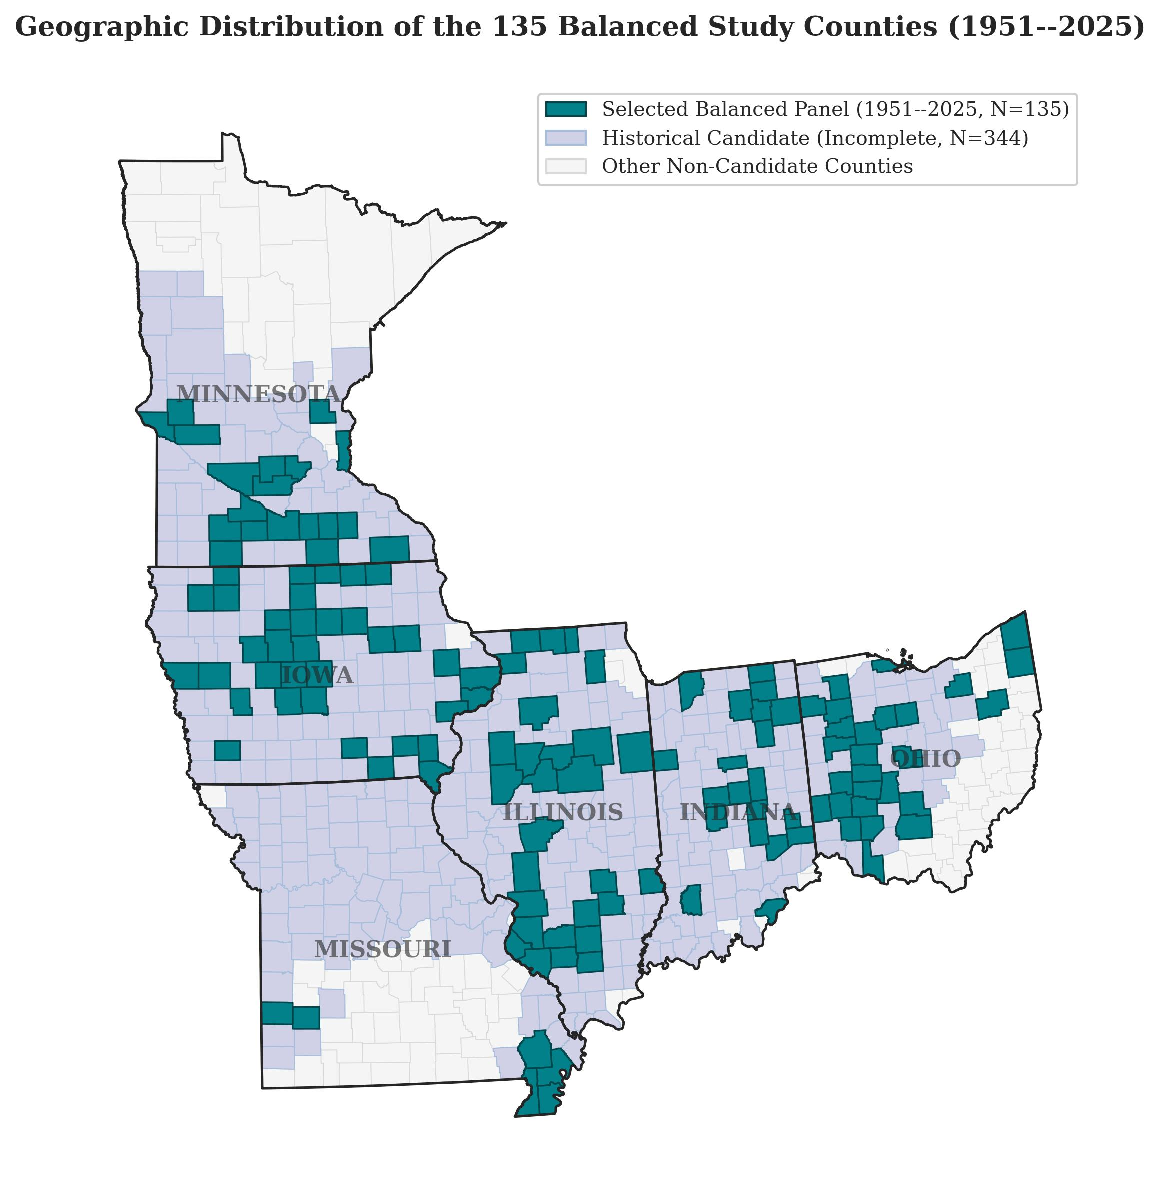
\includegraphics[width=0.92\textwidth]{figures/fig_study_area_map}
    \caption{Geographic distribution of the 135 balanced study counties across the six Midwestern states (1951--2025), illustrating balanced coverage across the primary agro-ecological subregions of the Corn and Soybean Belt.}
    \label{fig:study_area_map}
\end{figure}

\subsection{Soybean Phenology and Critical Agro-Climatic Sensitivity Windows}
\label{sec:data_phenology}

Soybean development spans approximately six months, initiating with sowing in late April or May and concluding with harvest in September or October \citep{FehrCaviness1977}. To capture how intra-seasonal meteorological anomalies propagate into realized yield shocks, the cultivation cycle is structured into four sequential operational and phenological phases:

\begin{enumerate}
    \item \textbf{Sowing, Germination, and Emergence (April--May):}
    Germination requires seedbed temperatures consistently above $10^\circ\text{C}$ along with adequate moisture for imbibition. While farmers aim to plant early (late April to early May) to maximize solar radiation capture during summer, prolonged exposure to saturated, cold soils ($<10^\circ\text{C}$) induces seed chilling injury, pathogen vulnerability, and soil compaction. Substantial planting delays into June compress the vegetative window and curtail overall yield potential.
    
    \item \textbf{Vegetative Growth and Canopy Closure (June, V1--Vn):}
    Following emergence, the crop undergoes rapid vegetative development, driven by thermal accumulation (Growing Degree Days, $GDD$), establishing trifoliate nodes and taproots into intermediate soil layers ($7$--$28\text{ cm}$). Moderate early moisture deficits encourage deeper root penetration, whereas severe drought or prolonged root-zone waterlogging stunting canopy closure permanently diminishes the photosynthetic capacity needed to support reproductive organs.
    
    \item \textbf{Mid-Summer Reproductive Peak and Pod-Filling (July--August, R1--R6):}
    The July--August window represents the critical biological bottleneck of the entire crop lifecycle \citep{Schlenker2009, Lobell2014}. In July (flowering and pod initiation, R1--R3), atmospheric maximum temperatures exceeding $30^\circ\text{C}$ and elevated vapor pressure deficits ($VPD > 1.5\text{ kPa}$) induce pollen sterility, reduce pollination efficiency, and trigger irreversible floral and pod abscission. In August (pod filling and seed enlargement, R4--R6), transpirational water demand peaks as assimilated carbon and nitrogen translocate into developing seeds. Severe heat or moisture deficits in August cause leaf senescence, pod abortion, and shriveled seeds, whereas abundant subsoil moisture and moderate temperatures maximize seed weight.
    
    \item \textbf{Maturation, Desiccation, and Harvest (September--October, R7--R8):}
    Upon reaching physiological maturity (R7), dry matter accumulation ceases, and seed moisture decreases from over $50\%$ toward harvest levels ($13\%$--$15\%$). Weather during this phase no longer influences biological yield potential, but dictates field workable days, combine efficiency, and mechanical harvest losses. Early hard autumn freezes ($T_{\text{min}} < 0^\circ\text{C}$) before R7 halt seed filling prematurely, while prolonged late-autumn rainfall induces lodging, pod shattering, and field access delays.
\end{enumerate}

\section{Exploratory Data Analysis of County Soybean Yields (1951--2025)}
\label{sec:data_eda}

\subsection{Secular Technological Trend, Productivity Tripling, and Anomaly Decomposition}
\label{sec:data_yield_decomposition}

To clarify the physical drivers of historical crop variation and formalize the empirical target, realized county soybean yield $y_{c,t}$ (bu/ac for county $c$ and year $t \in \{1951, \dots, 2025\}$) is decomposed into two orthogonal components:
\begin{equation}
    y_{c,t} = \tau_{c,t} + \epsilon_{c,t}
    \label{eq:yield_decomp_ch3}
\end{equation}
where $\tau_{c,t}$ represents the deterministic secular trend driven by cumulative technological, agronomic, and genetic innovations, and $\epsilon_{c,t}$ denotes the stochastic shock anomaly induced by intra-seasonal atmospheric forcing and environmental extremes.

\begin{figure}[htbp]
    \centering
    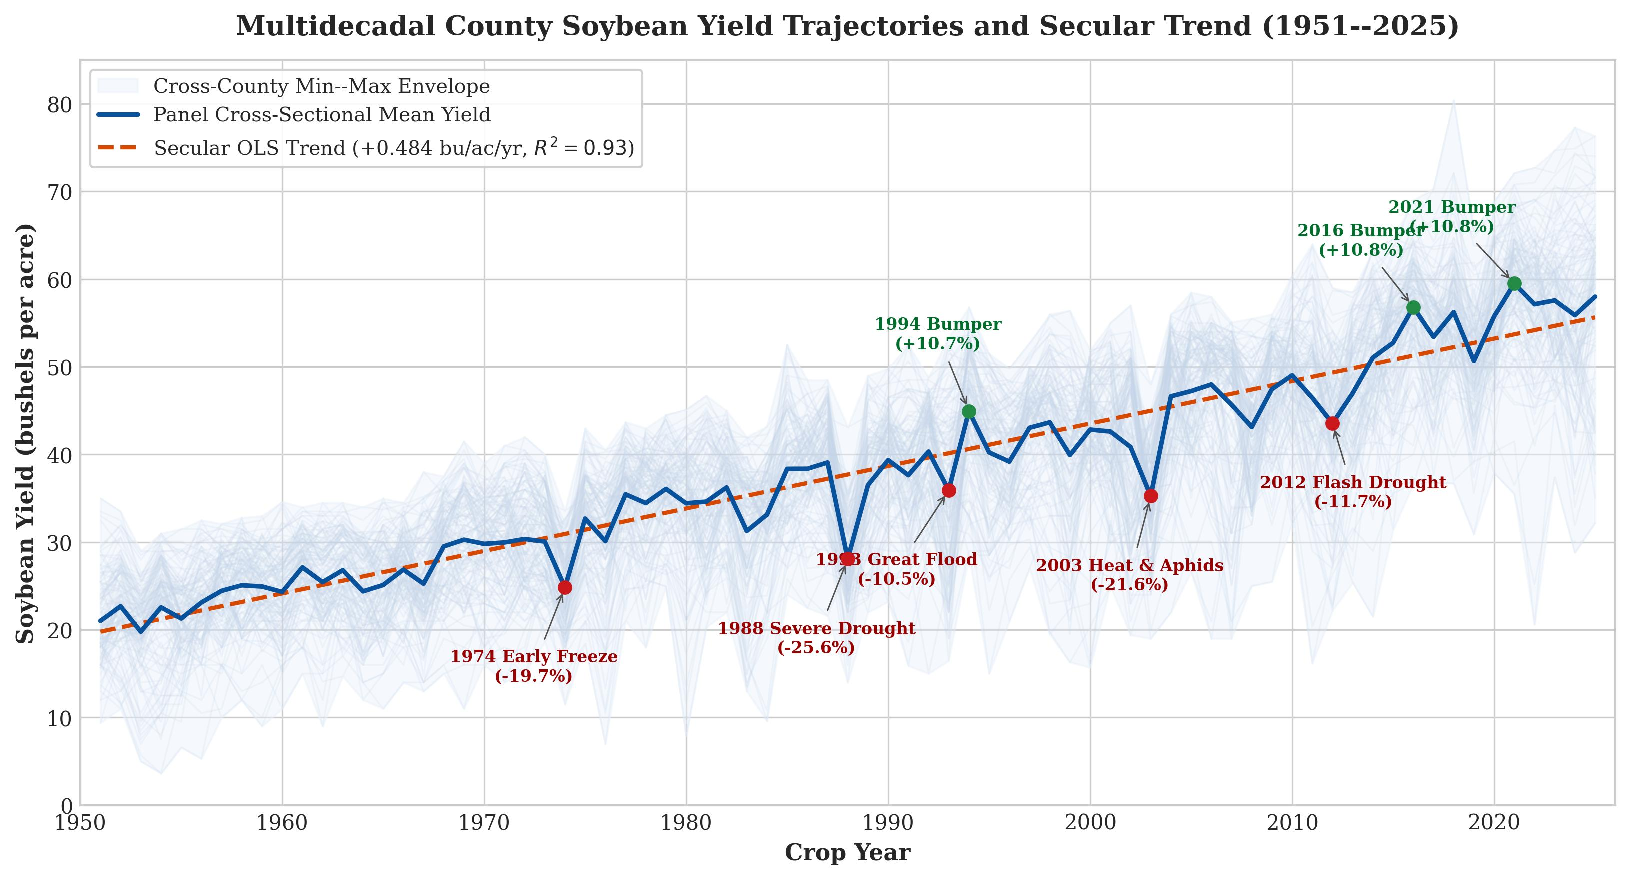
\includegraphics[width=0.96\textwidth]{figures/fig_yield_trajectory}
    \caption{Multidecadal county soybean yield trajectories and secular trend across 135 Midwestern counties (1951--2025). Light lines represent individual county histories; the solid blue line denotes the annual cross-sectional panel mean; the dashed line represents the secular OLS trend; and markers highlight major historical climatic shock anomalies.}
    \label{fig:yield_trajectory}
\end{figure}

The secular baseline $\tau_{c,t}$ captures steady technological progress, including breeding advancements (improved lodging resistance, optimized maturity groups), transgenic traits, farm mechanization, subsurface tile drainage, and precision crop inputs. Across the 75-year panel, regional soybean yields expanded from an unweighted mean of $22.77\text{ bu/ac}$ in the 1950s to $57.31\text{ bu/ac}$ in the 2020s, a net gain of $+151.7\%$ (Table~\ref{tab:decadal_yields}). A pooled linear secular trend accounts for over 81\% of total county-year yield variance ($R^2 = 0.8122$, $N = 10{,}125$). Aggregated to the annual regional mean ($N = 75$), an ordinary least squares regression yields an average rate of progress of $+0.484\text{ bu/ac/year}$ ($R^2 = 0.9323$):
\begin{equation}
    \hat{y}_t = 0.484 \cdot t - 925.46 \quad (t = 1951, \dots, 2025)
    \label{eq:panel_trend}
\end{equation}

% Table 3.2: Decadal Distributional Statistics of Soybean Yields (1951-2025)
\begin{table}[htbp]
\centering
\footnotesize
\setlength{\tabcolsep}{3.5pt}
\caption{Decadal distributional dynamics of Midwestern county-level soybean yields (1951--2025).}
\label{tab:decadal_yields}
\begin{tabular*}{\textwidth}{@{\extracolsep{\fill}}l c c c c c c c c}
\toprule
\textbf{Period} & \textbf{Obs.} & \textbf{Mean} & \textbf{Median} & \textbf{Std. Dev.} & \textbf{Min} & \textbf{Max} & \textbf{IQR} & \textbf{CV} \\
 & ($N$) & (bu/ac) & (bu/ac) & (bu/ac) & (bu/ac) & (bu/ac) & (bu/ac) & (\%) \\
\midrule
1950s (1951--1959) & 1,215 & 22.77 & 23.10 & 5.01 & 3.6 & 35.0 & 6.55 & 22.0\% \\
1960s (1960--1969) & 1,350 & 26.51 & 26.60 & 5.07 & 9.0 & 41.5 & 6.98 & 19.1\% \\
1970s (1970--1979) & 1,350 & 31.38 & 32.00 & 6.04 & 7.0 & 44.5 & 8.90 & 19.2\% \\
1980s (1980--1989) & 1,350 & 35.01 & 35.75 & 6.63 & 7.9 & 52.5 & 8.58 & 19.0\% \\
1990s (1990--1999) & 1,350 & 40.43 & 41.50 & 7.08 & 15.0 & 56.8 & 9.27 & 17.5\% \\
2000s (2000--2009) & 1,350 & 43.97 & 45.00 & 7.78 & 15.7 & 58.5 & 11.20 & 17.7\% \\
2010s (2010--2019) & 1,350 & 50.70 & 51.40 & 7.80 & 16.2 & 80.4 & 10.00 & 15.4\% \\
2020s (2020--2025) & 810 & 57.31 & 57.95 & 7.57 & 20.6 & 77.3 & 9.65 & 13.2\% \\
\midrule
\textbf{Full Panel (1951--2025)} & \textbf{10,125} & \textbf{37.72} & \textbf{36.70} & \textbf{12.40} & \textbf{3.6} & \textbf{80.4} & \textbf{19.00} & \textbf{32.9\%} \\
\bottomrule
\end{tabular*}
\vspace{1ex}
\raggedright
\footnotesize{\textit{Notes:} Yields are measured in bushels per acre (bu/ac). Obs. denotes total county-year observations in each period (135 counties $\times$ years). IQR is the interquartile range ($Q_3 - Q_1$). CV is the coefficient of variation ($100 \times \sigma / \mu$). Note the systematic decrease in CV from 22.0\% in the 1950s to 13.2\% in the 2020s despite an increase in absolute standard deviation.}
\end{table}


From a supply-chain and modeling perspective, separating $\tau_{c,t}$ from $\epsilon_{c,t}$ is crucial. While the secular trajectory is readily anticipated by market actors and capitalized into logistics capacity, systemic commodity volatility and supply shortfalls are driven by the weather-induced anomaly $\epsilon_{c,t}$. Furthermore, because baseline yields have nearly tripled, a given percentage drought shock corresponds to a substantially larger physical volume loss today than in the 1950s.

A deterministic linear specification provides a parsimonious, robust baseline that eliminates Runge-type endpoint oscillations and avoids overfitting the multi-year climate cycles that flexible non-parametric filters inadvertently absorb \citep{Schlenker2009, Lobell2014}. The formal mathematical estimation of candidate detrending models, penalization schemes, and strict train-only expanding-window implementations is formalized in the predictive methodology of Chapter~4.

\subsection{Spatial Heterogeneity and Regional Productivity Divergence}

While the secular trend is positive across the entire Midwest, regional productivity exhibits pronounced spatial heterogeneity across states and agro-climatic zones. Figure~\ref{fig:state_yield_distributions} contrasts the cross-sectional yield distributions and decadal trajectories across the six states.

\begin{figure}[htbp]
    \centering
    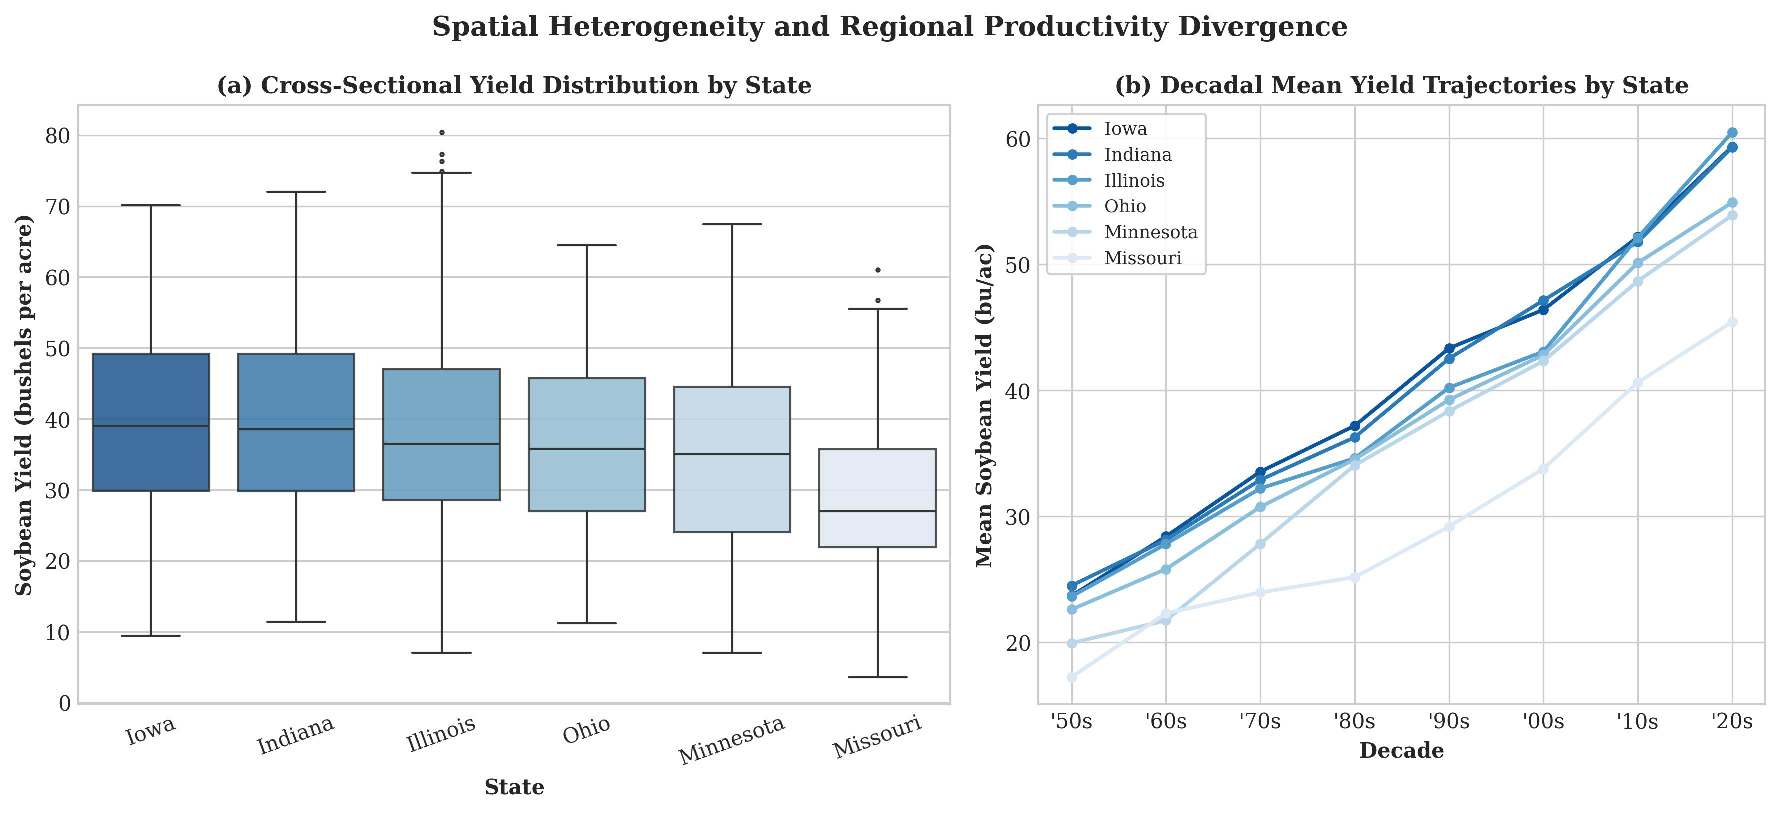
\includegraphics[width=0.96\textwidth]{figures/fig_state_yield_distributions}
    \caption{Spatial heterogeneity of county soybean yields: (a) cross-sectional yield distributions by state ordered by median yield; (b) decadal mean yield trajectories across the six Midwestern states from the 1950s to the 2020s.}
    \label{fig:state_yield_distributions}
\end{figure}

Iowa (mean yield $39.73\text{ bu/ac}$; secular trend $+0.495\text{ bu/ac/year}$) and Illinois (mean $38.35\text{ bu/ac}$; trend $+0.491\text{ bu/ac/year}$) form the high-yielding core of the Corn Belt, underpinned by deep prairie soils with superior moisture-retention capacities. Indiana ($39.52\text{ bu/ac}$) and western Ohio ($36.88\text{ bu/ac}$) exhibit comparable productivity with lower cross-county dispersion. 

In contrast, Minnesota presents a lower historical mean ($35.10\text{ bu/ac}$) but the fastest linear growth rate in the panel ($+0.509\text{ bu/ac/year}$). This rapid acceleration reflects the northward migration of soybean acreage during the late 20th century, made possible by the commercial development of cold-tolerant, short-season cultivars (maturity groups 0 and 00) and warmer spring temperatures. At the southern fringe, Missouri displays both the lowest historical yield level ($29.04\text{ bu/ac}$) and the lowest trend slope ($+0.386\text{ bu/ac/year}$), driven by shallower topsoils (claypan subsoils) and elevated susceptibility to summer heatwaves and dry spells.

\subsection{Dispersion Dynamics: Absolute Variance vs. Relative Volatility}

A fundamental question in agricultural risk analysis is whether technological modernization has altered crop vulnerability to environmental shocks. Figure~\ref{fig:dispersion_dynamics} resolves this by examining absolute cross-county standard deviation ($\sigma_t$) alongside relative volatility, measured by the coefficient of variation ($CV_t = 100 \times \sigma_t / \mu_t$).

\begin{figure}[htbp]
    \centering
    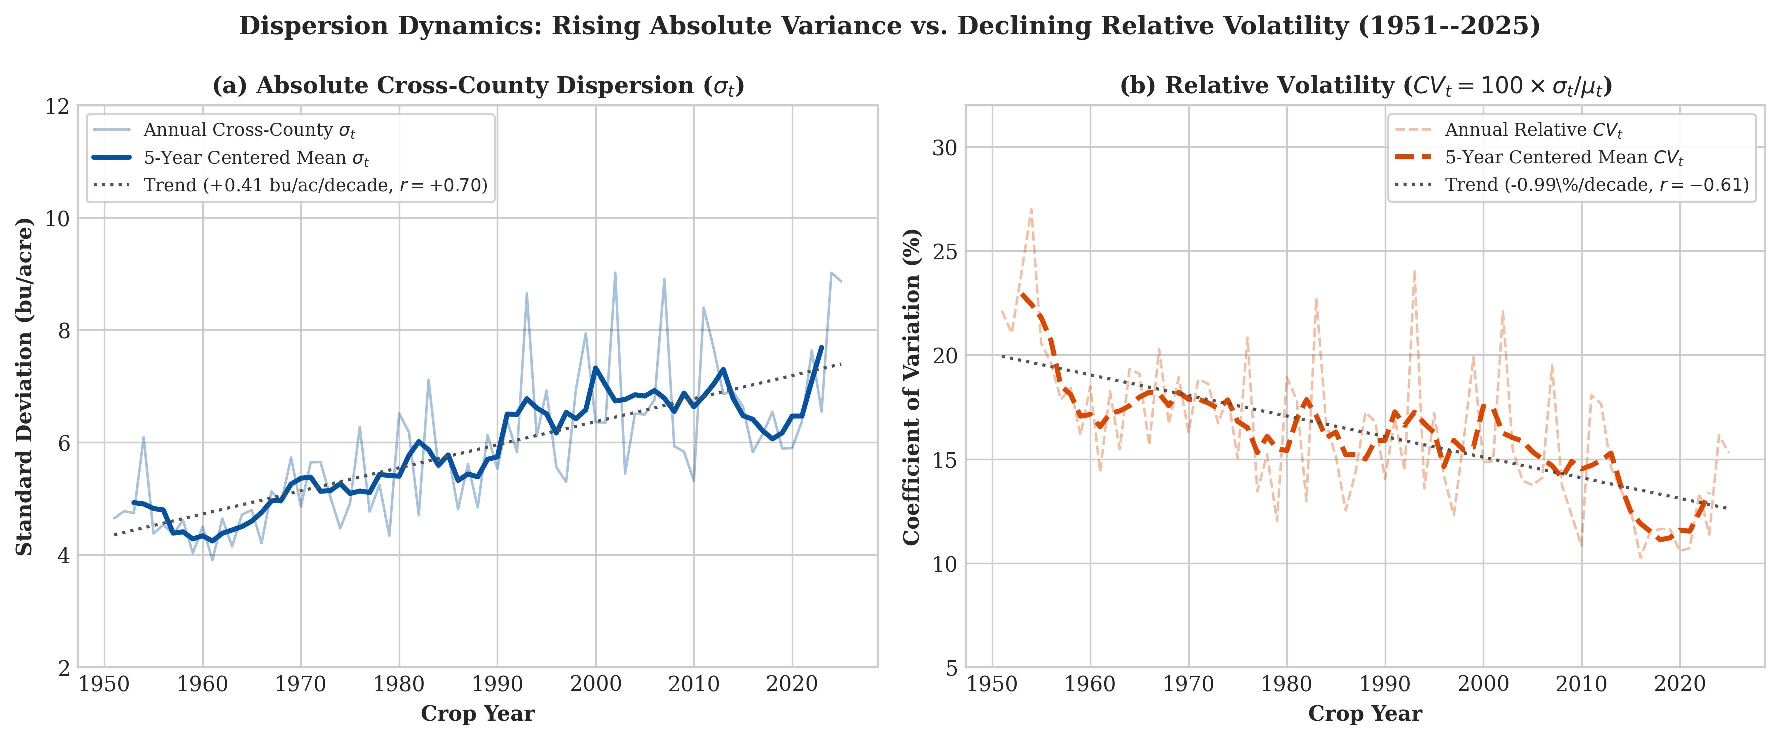
\includegraphics[width=0.90\textwidth]{figures/fig_dispersion_dynamics}
    \caption{Dispersion dynamics across the 135 Midwestern study counties (1951--2025). The blue curves illustrate rising absolute cross-county standard deviation ($\sigma_t$, left axis), while the dashed orange curves depict steadily declining relative coefficient of variation ($CV_t$, right axis). Solid thick lines denote 5-year centered rolling averages.}
    \label{fig:dispersion_dynamics}
\end{figure}

The empirical evidence reveals a clear dichotomy: while absolute standard deviation has expanded from $5.01\text{ bu/ac}$ in the 1950s to $7.57\text{ bu/ac}$ in the 2020s ($r = +0.705$), the coefficient of variation has declined systematically from $22.0\%$ to $13.2\%$ ($r = -0.610$, Table~\ref{tab:decadal_yields}). Modern cultivars, seed treatments, and drainage have dampened \textit{relative} vulnerability to localized micro-stresses. However, because baseline yield levels have nearly tripled, the \textit{absolute} bushel shortfall generated during severe regional droughts is substantially larger today, heightening volume exposure for commercial supply-chain logistics.

\subsection{Macro-Climatic Historical Yield Shocks and Biological Asymmetry}
\label{sec:data_yield_shocks}

The 75-year panel captures prominent macro-climatic shock campaigns that serve as out-of-sample benchmark years. Using an asymmetric anomaly threshold of $|\epsilon_t / \hat{y}_t| \ge 10\%$ relative to the secular trend, Table~\ref{tab:yield_shocks} classifies historical extreme campaigns into adverse shortfalls and favorable bumper regimes alongside their dominant hazard archetypes.

% Table 3.3: Historical Macro-Climatic Yield Shocks in the Midwestern Panel (1951-2025)
\begin{table}[htbp]
\centering
\small
\caption{Historical macro-climatic shock years and associated meteorological drivers (1951--2025).}
\label{tab:yield_shocks}
\begin{tabularx}{\textwidth}{c c c c c X}
\toprule
\textbf{Year} & \textbf{Observed} & \textbf{Trend} & \textbf{Anomaly} & \textbf{Rel. Anomaly} & \textbf{Primary Meteorological / Ecological Driver} \\
 & (bu/ac) & (bu/ac) & (bu/ac) & (\%) & \\
\midrule
\multicolumn{6}{l}{\textit{\textbf{Panel A: Major Adverse Macro-Climatic Yield Shocks (Negative Anomalies)}}} \\[0.5ex]
1988 & 28.08 & 37.72 & -9.64 & -25.6\% & Historic severe summer drought and persistent heatwave across the Corn Belt. \\
2003 & 35.26 & 44.98 & -9.72 & -21.6\% & Late-summer heat and moisture stress compounded by widespread soybean aphid outbreak. \\
1974 & 24.84 & 30.93 & -6.09 & -19.7\% & Excessively wet spring delaying planting, followed by mid-summer drought and early September frost. \\
2012 & 43.55 & 49.34 & -5.80 & -11.7\% & Extensive summer flash drought and record July heat across the central United States. \\
1983 & 31.27 & 35.29 & -4.02 & -11.4\% & Prolonged July-August heatwave and severe drought across the Corn and Soybean Belt. \\
1993 & 35.92 & 40.14 & -4.22 & -10.5\% & Great Upper Mississippi River flood; prolonged waterlogging, root asphyxia, and disease. \\
\midrule
\multicolumn{6}{l}{\textit{\textbf{Panel B: Prominent Favorable Bumper Harvests (Positive Anomalies)}}} \\[0.5ex]
1952 & 22.69 & 20.27 & +2.41 & +11.9\% & Exceptionally favorable vegetative and pod-filling moisture across the central belt. \\
2021 & 59.50 & 53.70 & +5.79 & +10.8\% & Optimal reproductive rainfall and moderate temperatures throughout August. \\
2016 & 56.81 & 51.28 & +5.53 & +10.8\% & Broadly distributed summer rains and minimal extreme heat stress across the Midwest. \\
1994 & 44.95 & 40.62 & +4.33 & +10.7\% & Record-setting benign growing conditions with timely August rains and cool nights. \\
\bottomrule
\end{tabularx}
\vspace{1ex}
\raggedright
\footnotesize{\textit{Notes:} Observed represents the unweighted cross-sectional mean yield of all 135 panel counties. Trend is estimated via linear OLS over 1951--2025 ($\hat{y}_t = 0.484t - 925.46$). Anomaly is $y_t - \hat{y}_t$, and Rel. Anomaly is $(y_t - \hat{y}_t)/\hat{y}_t \times 100$. Note that 1988 represents the deepest shortfall in the 75-year record ($-25.6\%$), while 1993 highlights non-drought atmospheric hazards (excess precipitation and soil saturation).}
\end{table}


The empirical distribution of extreme yield anomalies exhibits pronounced \textbf{biological and statistical asymmetry}. Favorable bumper harvests cluster tightly within a narrow upper bound ($+10.1\%$ to $+11.9\%$; e.g., 1952, 1961, 1994, 2016, 2021). Under optimal weather, dry matter accumulation is bounded by an asymptotic physiological ceiling governed by RuBisCO carboxylation kinetics, canopy radiation interception, and genetic sink strength. 

Conversely, adverse abiotic stressors possess no physiological floor short of total crop loss, generating an elongated lower tail down to $-19.7\%$ (1974), $-21.6\%$ (2003), and $-25.6\%$ (1988), producing significant negative skewness ($-1.12$, Jarque-Bera test $p < 0.001$). As cataloged in Table~\ref{tab:yield_shocks}, these severe downside shocks reflect distinct compound hazards:
\begin{itemize}
    \item \textit{Compound Thermal-Drought Stress (1953, 1983, 1988, 2012):} High temperatures ($T_{\text{max}} > 30^\circ\text{C}$ and $>35^\circ\text{C}$) coupled with elevated vapor pressure deficits ($VPD > 1.8\text{ kPa}$) induce pollen sterility, floral abscission, and transpirational collapse \citep{Schlenker2009, Lobell2014}.
    \item \textit{Pluvial Inundation and Soil Anoxia (1993):} Persistent waterlogging causes root-zone oxygen deprivation, impairs symbiotic nitrogen fixation, and fosters fungal diseases, cutting yields by $-10.5\%$ in the absence of drought.
    \item \textit{Planting Delays and Early Frost (1974):} Wet spring conditions delay planting into June, pushing pod fill late into summer and exposing immature crops to early autumn freezes ($-19.7\%$).
    \item \textit{Compound Biotic-Abiotic Stress (2003):} Late-summer moisture deficits interact synergistically with aphid outbreaks, exacerbating losses ($-21.6\%$).
\end{itemize}

Crucially, because synoptic weather patterns span hundreds of kilometers, meteorological anomalies affect contiguous counties simultaneously. Within our panel, cross-county detrended yield correlations average above $0.75$, highlighting strong spatial autocorrelation and necessitating strict year-based temporal cross-validation to prevent spatial leakage \citep{Sweetetal2023}.

% ==============================================================================
% PART 2: ATMOSPHERIC REANALYSIS AND AGRO-CLIMATIC SENSITIVITY
% ==============================================================================

\section{Atmospheric Reanalysis: ECMWF ERA5-Land}
\label{sec:data_era5}

\subsection{Methodological Rationale for a Weather-Only Scope}
\label{sec:data_weather_only_rationale}

The empirical predictive framework restricts dynamic predictive inputs strictly to gridded surface weather from ECMWF ERA5-Land \citep{MunozSabater2021}, which provides continuous, physically consistent hourly meteorological fields at $0.1^\circ \times 0.1^\circ$ resolution ($\approx 9\text{ km}$ across the Midwest), free from station-discontinuation artifacts and spatial interpolation gaps.

As theoretically grounded in Chapter~\ref{chap:literature_review}, this weather-only constraint is dictated by operational real-time requirements and multidecadal data integrity:
\begin{enumerate}
    \item \textbf{Operational Feasibility and Lag Elimination:} County-level management records (planting dates, fertilizer rates, cultivar adoptions) are compiled ex-post and released months after harvest, making them inadmissible for real-time forecasting. Furthermore, consistent 75-year historical records do not exist.
    \item \textbf{Historical Depth and Satellite Latency:} Remote sensing greenness proxies (MODIS/Sentinel NDVI, EVI, SIF) are available only post-2000, preventing multidecadal sampling of climatic extremes. Moreover, optical indices exhibit severe physiological latency, offering no predictive utility during pre-sowing and early vegetative windows ($H \ge 4$).
    \item \textbf{Zero Temporal Variance of Static Soil Grids:} While soil properties (SSURGO available water capacity, texture) help establish spatial baseline productivity, their values are temporally invariant ($\text{Var}(X_{it}) = 0$) and cannot explain interannual yield shocks.
    \item \textbf{Unconfounded Physical Benchmark:} Coupling yield models with dynamical seasonal climate forecasts (e.g., SEAS5) conflates crop response functions with climate model forecast drift and systematic biases. Restricting inputs to realized surface reanalysis establishes the empirical upper bound of predictability attributable strictly to observed atmospheric forcing up to each forecast cutoff.
\end{enumerate}

\subsection{Spatial Aggregation: Exact Planar Polygon Intersection}

To map gridded reanalysis fields into irregularly shaped administrative county polygons, an exact planar polygon-intersection geometry was computed (\texttt{spatial\_weights.csv}). Across the 135 counties and the ERA5-Land $0.1^\circ$ grid, 3,344 unique intersection polygons are identified with normalized area weights:
\begin{equation}
    w_{c,g} = \frac{\text{Area}(c \cap g)}{\text{Area}(c)}, \quad \sum_{g \in \mathcal{G}_c} w_{c,g} = 1
    \label{eq:spatial_weight}
\end{equation}
where $\text{Area}(c \cap g)$ is the planar intersection area between county polygon $c$ and grid cell $g$, and $\mathcal{G}_c$ denotes the set of intersecting grid cells.

This area-weighted polygon integration represents a significant methodological advance over naive centroid sampling. Centroid extraction assumes that a single point can represent an entire county, which introduces severe spatial sampling errors in large Midwestern counties characterized by localized convective precipitation gradients and heterogeneous topography. Exact area weighting accurately integrates the total atmospheric mass, radiation, and precipitation volume falling within county boundaries.

\subsection{Temporal Aggregation and Crop Campaign Structure}

Hourly ERA5-Land reanalysis fields are spatially aggregated via Equation~\eqref{eq:spatial_weight} and summarized into daily indicators:
\begin{itemize}
    \item \textbf{Thermodynamic States:} Daily mean, maximum, and minimum 2m air temperature ($T_{\text{mean}}, T_{\text{max}}, T_{\text{min}}$), daily mean 2m dewpoint ($T_{\text{dew}}$), and daily mean/maximum skin temperature ($T_{\text{skt}}$) in $^\circ$C.
    \item \textbf{Cumulative Fluxes:} Daily cumulative precipitation ($P$, mm/day), surface solar radiation downwards ($SSRD$, $\text{MJ}/\text{m}^2/\text{day}$), and surface thermal radiation downwards ($STRD$, $\text{MJ}/\text{m}^2/\text{day}$).
    \item \textbf{Boundary Layer and Wind Dynamics:} Daily mean surface pressure ($SP$, kPa), 10m horizontal wind components ($u_{10}, v_{10}$, m/s), and scalar wind speed ($WS_{10}$, m/s).
    \item \textbf{Pedological State Variables:} Daily mean soil temperature across four discrete depth horizons ($STL_1$--$STL_4$: $0$--$7$, $7$--$28$, $28$--$100$, and $100$--$289\text{ cm}$, $^\circ$C), and volumetric soil moisture across the same four horizons ($SM_1$--$SM_4$, $\text{m}^3/\text{m}^3$).
\end{itemize}

For each crop year $Y$, daily weather processing is structured over a 13-month campaign spanning from October 1 of year $Y-1$ to October 31 of year $Y$ (397 consecutive days). This multi-month temporal structure aligns with the 12 progressive monthly forecast horizons ($H=12, \dots, 1$) evaluated on the last day of each month, capturing antecedent overwinter soil moisture recharge and growing-season atmospheric forcing without temporal data leakage.

\subsection{Derived Agrometeorological Variables and Bioclimatic Indicators}
\label{sec:data_derived_weather}

Because crop physiological response functions operate non-linearly on compound atmospheric-hydrological demands rather than isolated averages \citep{Schlenker2009, Hoffman2020}, raw ERA5-Land fields are processed into primary and derived daily agrometeorological indicators (Table~\ref{tab:weather_variables}).

\begin{table}[htbp]
\centering
\footnotesize
\setlength{\tabcolsep}{4pt}
\renewcommand{\arraystretch}{1.15}
\caption{ERA5-Land surface meteorological variables and derived daily agrometeorological indicators.}
\label{tab:weather_variables}
\begin{tabularx}{\textwidth}{p{2.3cm} p{2.8cm} p{1.3cm} X}
\toprule
\textbf{Category} & \textbf{Symbol} & \textbf{Unit} & \textbf{Physical Description and Agronomic Rationale} \\
\midrule
\multicolumn{4}{l}{\textit{Panel A: Primary Atmospheric and Land-Surface Reanalysis Fields (ECMWF ERA5-Land)}} \\
Thermal Dynamics & $T_{\text{mean}}, T_{\text{max}}, T_{\text{min}}$ & $^\circ$C & Daily mean, maximum, and minimum 2\,m air temperature; thermal accumulation and heat stress. \\
& $T_{\text{dew}}$ & $^\circ$C & Daily mean 2\,m dewpoint temperature; near-surface moisture baseline. \\
Hydrological Fluxes & $P$ & mm/d & Total daily precipitation; surface water supply, recharge, and waterlogging. \\
& $PE$ & mm/d & Potential evaporation; atmospheric evaporative capacity from the surface. \\
Radiative Forcing & $SSRD$ & $\text{MJ}/\text{m}^2/\text{d}$ & Surface downward solar radiation; photosynthetically active radiation driving biomass assimilation. \\
Pedological Moisture & $SM_1, SM_2, SM_3$ & $\text{m}^3/\text{m}^3$ & Volumetric soil water across depths: $0$--$7\text{ cm}$ (seedbed), $7$--$28\text{ cm}$ (upper root zone), and $28$--$100\text{ cm}$ (deep root reservoir). \\
\midrule
\multicolumn{4}{l}{\textit{Panel B: Derived Agrometeorological and Bioclimatic Indicators}} \\
Evaporative Demand & $VPD$ & kPa & Vapor pressure deficit $e_s(T_{\text{mean}}) - e_a(T_{\text{dew}})$; atmospheric drying power driving stomatal closure. \\
Crop Water Demand & $ET_0$ & mm/d & FAO-56 Penman-Monteith reference evapotranspiration \citep{Allen1998}. \\
Climatic Balance & $P - ET_0$ & mm/d & Climatic water balance; net daily atmospheric moisture deficit or surplus. \\
Thermal Pacing & $GDD$ & $^\circ$C$\cdot$d & Growing Degree Days ($10$--$30^\circ$C); vegetative and reproductive phenological progression pacing. \\
Extreme Heat Stress & $HD_{30}, HD_{35}$ & binary & Daily heat day exceedances $\mathbb{I}(T_{\text{max}} \ge 30^\circ\text{C})$ and $\ge 35^\circ\text{C}$ \citep{Schlenker2009}. \\
Root-Zone Reservoir & $SM_{\text{root}}$ & $\text{m}^3/\text{m}^3$ & Depth-weighted soil water column ($0$--$100\text{ cm}$, Eq.~\eqref{eq:sm_root}); multi-month hydrological buffer. \\
\bottomrule
\end{tabularx}
\end{table}


\paragraph{Vapor Pressure Deficit ($VPD$).} Atmospheric evaporative demand is parameterized via Vapor Pressure Deficit, which quantifies the drying power of the air. Saturation vapor pressure $e_s(T_{\text{mean}})$ and actual vapor pressure $e_a(T_{\text{dew}})$ (in kPa) are computed via Tetens formulations:
\begin{align}
    e_s(T_{\text{mean}}) &= 0.61078 \exp\left( \frac{17.27 \, T_{\text{mean}}}{T_{\text{mean}} + 237.3} \right), \quad
    e_a(T_{\text{dew}}) = 0.61078 \exp\left( \frac{17.27 \, T_{\text{dew}}}{T_{\text{dew}} + 237.3} \right) \label{eq:tetens} \\
    VPD &= \max\left(0, \, e_s(T_{\text{mean}}) - e_a(T_{\text{dew}})\right) \label{eq:vpd}
\end{align}
Elevated $VPD$ ($>1.5\text{ kPa}$) triggers stomatal closure to prevent xylem cavitation, suppressing transpirational cooling and carbon assimilation during reproductive stages \citep{Grossiord2020, Lobell2014}.

\paragraph{Reference Evapotranspiration ($ET_0$) and Climatic Water Balance ($P - ET_0$).} Potential atmospheric water demand is modeled via the standardized FAO-56 Penman-Monteith equation for a short grass reference canopy \citep{Allen1998}:
\begin{equation}
    ET_0 = \frac{0.408 \, \Delta \, (R_n - G) + \gamma \, \frac{900}{T_{\text{mean}} + 273} \, u_2 \, (e_s - e_a)}{\Delta + \gamma \, (1 + 0.34 \, u_2)}
    \label{eq:penman_monteith}
\end{equation}
where $R_n$ is net surface radiation ($\text{MJ}/\text{m}^2/\text{day}$), $G \approx 0$ is daily soil heat flux density, $u_2$ is 2m wind speed ($\text{m/s}$), $\Delta$ is the saturation vapor pressure slope, and $\gamma$ is the psychrometric constant. Daily climatic water balance tracks atmospheric moisture deficits or recharge surpluses:
\begin{equation}
    P_{\text{net}} = P - ET_0
    \label{eq:climatic_balance}
\end{equation}

\paragraph{Thermal Pacing and Extreme Heat Days ($GDD, HD_{30}, HD_{35}$).} Phenological progression is tracked through Growing Degree Days ($GDD$, base $10^\circ\text{C}$, cap $30^\circ\text{C}$):
\begin{equation}
    GDD = \max\left(0, \, \frac{\min(T_{\text{max}}, 30) + \max(T_{\text{min}}, 10)}{2} - 10\right)
    \label{eq:gdd}
\end{equation}
To capture non-linear thermal damage thresholds \citep{Schlenker2009}, extreme heat exposure is quantified via daily exceedances:
\begin{equation}
    HD_{30} = \max(0, \, T_{\text{max}} - 30), \quad HD_{35} = \max(0, \, T_{\text{max}} - 35)
    \label{eq:heat_days}
\end{equation}
alongside binary daily occurrences $\mathbb{I}(T_{\text{max}} \ge 30^\circ\text{C})$ and $\mathbb{I}(T_{\text{max}} \ge 35^\circ\text{C})$.

\paragraph{Integrated Root-Zone Soil Moisture ($SM_{\text{root}}$).} Volumetric soil moisture across discrete depth horizons is aggregated into an integrated column accessible to mature soybean taproots ($0$--$100\text{ cm}$):
\begin{equation}
    SM_{\text{root}} = 0.07 \, SM_1 + 0.21 \, SM_2 + 0.72 \, SM_3
    \label{eq:sm_root}
\end{equation}
weighting by layer thickness ($7\text{ cm}$, $21\text{ cm}$, $72\text{ cm}$). This metric buffers transient surface dry spells and tracks subsoil moisture memory sustaining transpirational uptake during summer rainfall deficits \citep{Vijverberg2023}.

\section{Exploratory Agro-Climatic Analysis and Yield Sensitivity}
\label{sec:data_climate_eda}

\subsection{Baseline Climatology and Intra-Annual Seasonality}
\label{sec:data_seasonality}

Before examining multi-decadal historical shocks, it is essential to establish the intra-annual baseline climatology that governs crop development across the Midwestern Corn Belt. Utilizing the daily spatially weighted ERA5-Land reanalysis across the 135 study counties over the 1950--present record, Figure~\ref{fig:weather_seasonality} characterizes the seasonal progression of thermal regimes, cumulative water balances, and edaphic moisture depletion across the primary soybean growing cycle (April 1 to October 31).

\begin{figure}[htbp]
    \centering
    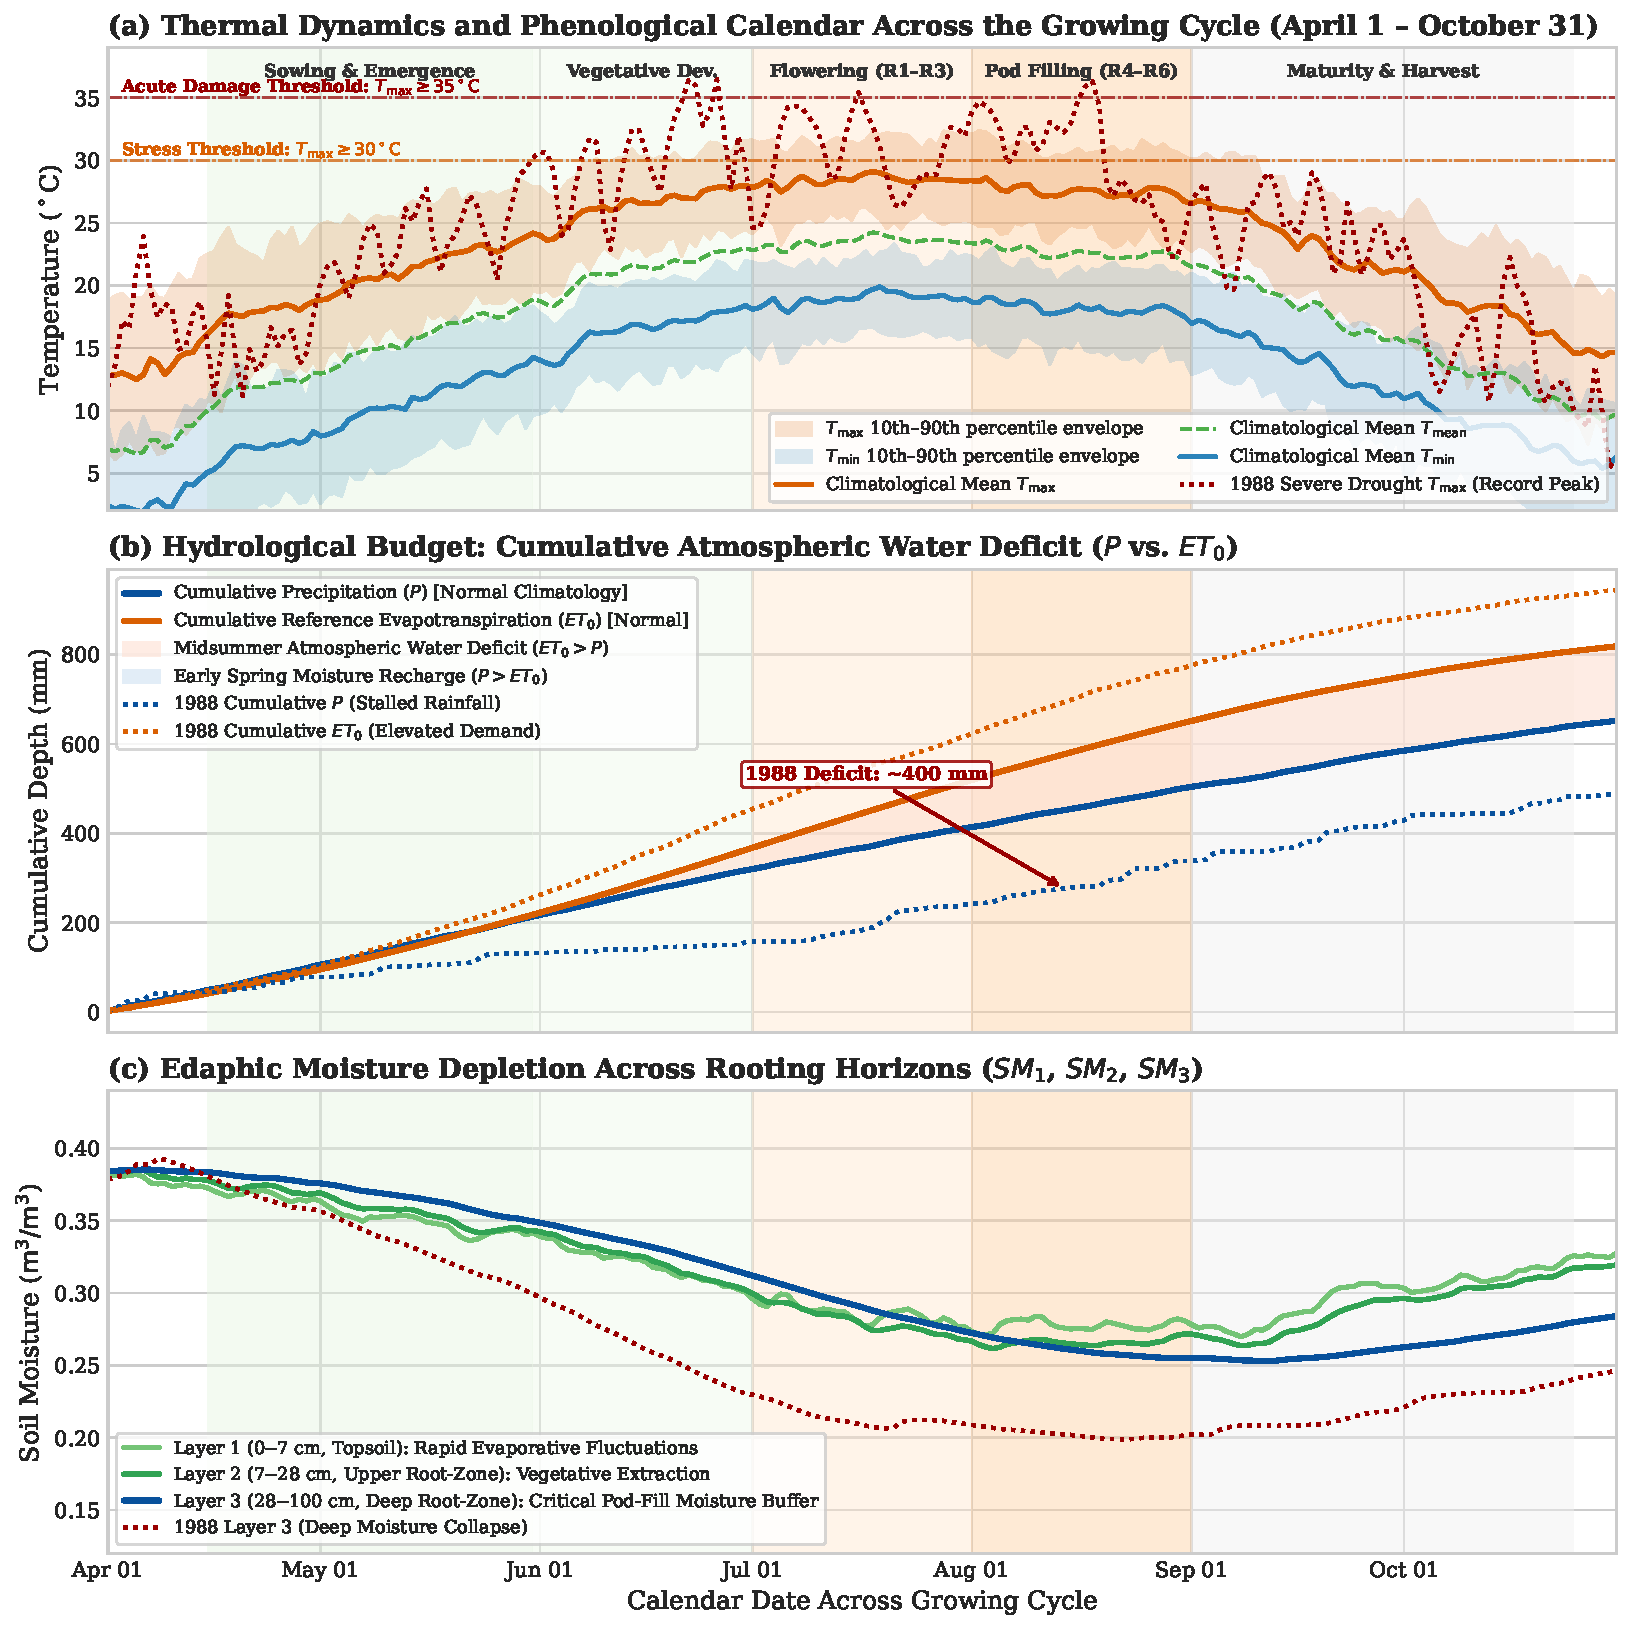
\includegraphics[width=0.96\textwidth]{figures/fig_weather_seasonality}
    \caption{Midwestern agro-climatic seasonality and intra-annual phenological dynamics across the 135 study counties (April 1 to October 31). Panel (a) illustrates daily thermal dynamics ($T_{\text{max}}, T_{\text{mean}}, T_{\text{min}}$) alongside 10th--90th percentile envelopes and cardinal damage thresholds ($30^\circ\text{C}$ and $35^\circ\text{C}$), contrasted against the record 1988 severe drought. Vertical shaded bands demarcate the five standardized phenological development stages. Panel (b) depicts the cumulative hydrological budget, highlighting the emergence of the midsummer atmospheric water deficit ($ET_0 > P$) in July and August. Panel (c) tracks volumetric soil moisture depletion across discrete rooting horizons ($SM_1$, $SM_2$, $SM_3$), demonstrating the essential buffering capacity of the deep root zone ($28$--$100\text{ cm}$).}
    \label{fig:weather_seasonality}
\end{figure}

The empirical intra-annual climatology synthesizes three foundational agronomic mechanisms across the developmental windows established in Section~\ref{sec:data_phenology}:

First, daily thermal progression (Figure~\ref{fig:weather_seasonality}a) aligns with the biological cardinal boundaries of the soybean plant. During the pre-sowing and emergence window (April 15--May 31), mean ambient temperatures rise from $8^\circ\text{C}$ to $18^\circ\text{C}$, safely exceeding the biological base germination threshold ($T_{\text{base}} = 10^\circ\text{C}$). Across the 75-year climatological record (1951--2025), summer maximum temperatures ($T_{\text{max}}$) peak in mid-July at $28.5^\circ\text{C}$ with an interdecile envelope bounded between $24^\circ\text{C}$ and $32^\circ\text{C}$. In contrast, during historical drought cohorts—exemplified by 1953, 1983, 1988, and 2012—daily maxima consistently pierced above the $30^\circ\text{C}$ floral abortion threshold and repeatedly exceeded the $35^\circ\text{C}$ acute damage ceiling throughout flowering (R1--R3) and early pod set. Conversely, during prominent bumper harvest cohorts such as 1952, 1961, 1994, 2016, and 2021, summer maxima remained consistently mild (hovering between $25^\circ\text{C}$ and $28^\circ\text{C}$), completely preventing canopy heat stress.

Second, the cumulative hydrological budget (Figure~\ref{fig:weather_seasonality}b) reveals the emergence of a structural midsummer atmospheric water deficit. In early spring (April and May), cumulative precipitation ($P \approx 200\text{ mm}$) exceeds reference crop evapotranspiration ($ET_0 \approx 180\text{ mm}$), ensuring robust topsoil recharge. However, starting in mid-June and accelerating throughout July and August, rising net radiation and vapor pressure deficits drive cumulative $ET_0$ to surge past cumulative rainfall. Under normal climatological conditions, a net seasonal atmospheric moisture deficit of $\approx 180\text{ mm}$ opens between $ET_0$ ($820\text{ mm}$) and $P$ ($640\text{ mm}$). During acute drought events like 1988 and 2012, rainfall stalled at barely $400$--$450\text{ mm}$ while evaporative demand exceeded $920\text{ mm}$, opening an unprecedented atmospheric moisture deficit of over $400\text{ mm}$. In contrast, bumper campaigns benefit from timely, well-distributed convective rainfall events that maintain cumulative deficits near a moderate equilibrium.

Third, the edaphic moisture profile (Figure~\ref{fig:weather_seasonality}c) demonstrates the critical buffering role of deep soil horizons. Volumetric moisture in the thin topsoil layer ($SM_1$, $0$--$7\text{ cm}$) exhibits erratic, high-frequency fluctuations driven by individual convective precipitation pulses and rapid surface evaporation. The intermediate layer ($SM_2$, $7$--$28\text{ cm}$) undergoes rapid extraction during vegetative expansion in June. Consequently, during the critical reproductive pod-filling phase in August (R4--R6), the crop becomes overwhelmingly reliant on the deep root-zone moisture reservoir ($SM_3$, $28$--$100\text{ cm}$). In normal seasons and bumper years, $SM_3$ declines smoothly from $0.38$ to $0.26\text{ m}^3/\text{m}^3$, providing a stable moisture buffer. In severe drought campaigns (such as 1988 and 1983), transpirational demand completely depleted $SM_3$ down to $0.18\text{ m}^3/\text{m}^3$, driving the soil column near the permanent wilting point and inducing widespread canopy desiccation.

\subsection{Historical Agro-Climatic Stress and the Yield Shock Nexus (1950--Present)}
\label{sec:data_climatology}

While intra-annual seasonality describes the average seasonal trajectory, interannual yield volatility is governed by the occurrence of acute atmospheric shocks. Figure~\ref{fig:weather_climatology} synchronizes the 75-year panel yield anomalies with the multi-decadal time series of atmospheric heat stress and evaporative demand across the 135 study counties.

\begin{figure}[htbp]
    \centering
    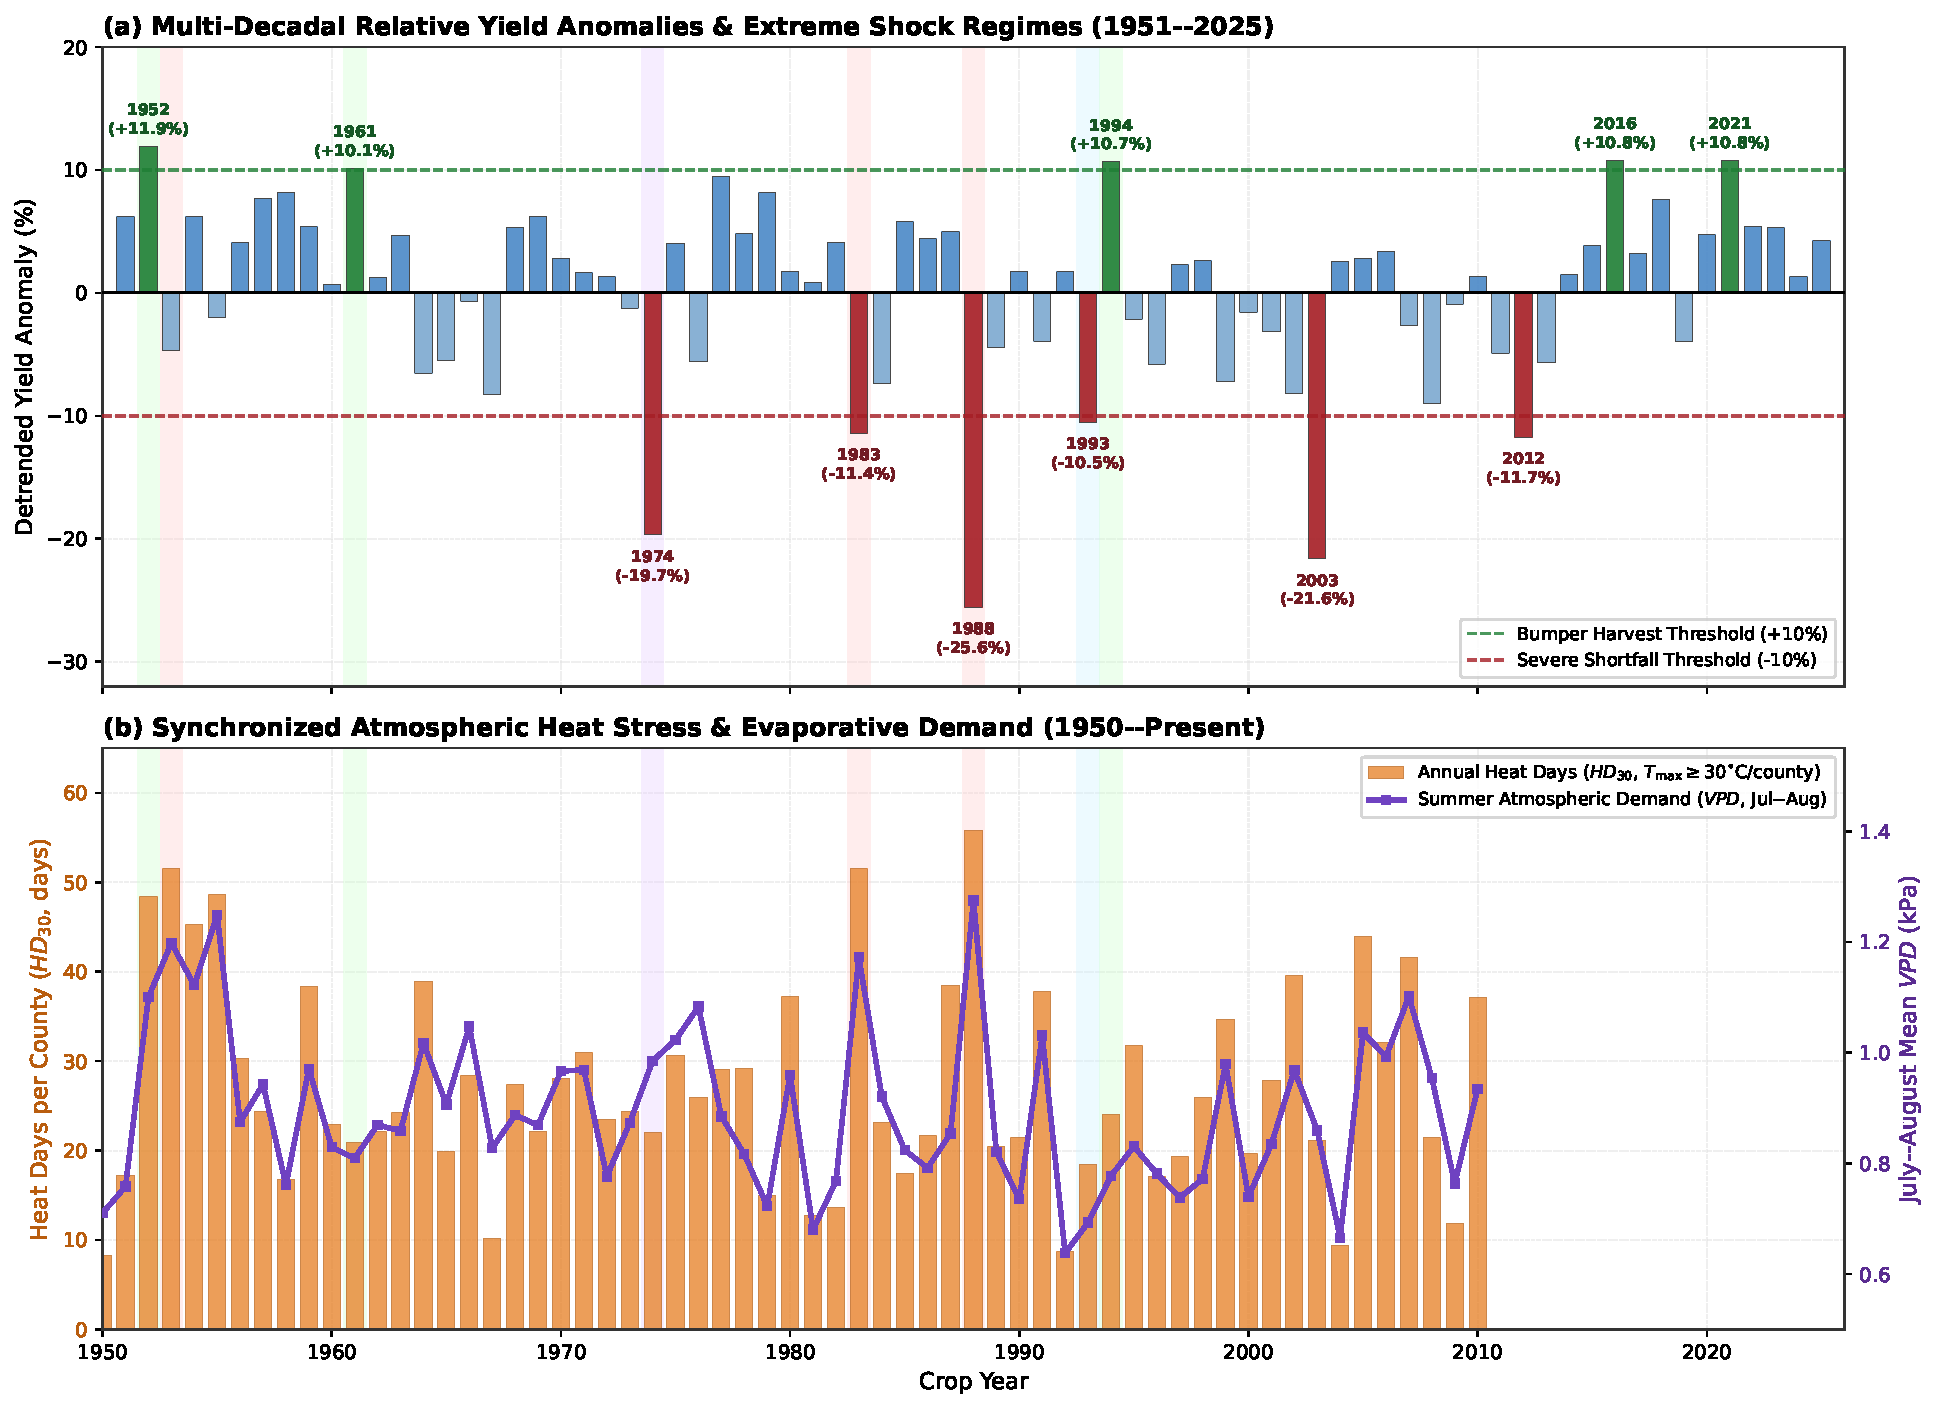
\includegraphics[width=0.96\textwidth]{figures/fig_weather_climatology}
    \caption{Multi-decadal agro-climatic stress evolution and county soybean yield shock nexus across 135 Midwestern study counties (1950--present). Panel (a) illustrates annual cross-sectional detrended yield anomalies relative to the secular linear trend, with prominent bumper harvests highlighted in emerald green ($\ge +10\%$) and catastrophic negative shortfalls in deep crimson ($\le -10\%$), bounded by explicit $\pm 10\%$ threshold guide lines. Panel (b) depicts annual extreme heat stress days ($HD_{30}$, days with $T_{\text{max}} \ge 30^\circ\text{C}$ per county, orange bars) and summer vapor pressure deficit ($VPD$, July--August mean, purple curve on secondary axis). Shaded vertical guide bands connect extreme anomaly years directly between panels, highlighting distinct thermal, hydrological, and biotic hazard mechanisms.}
    \label{fig:weather_climatology}
\end{figure}

The synchronized historical record resolves two foundational macro-climatic insights across the 75-year panel:

First, the most catastrophic regional harvest failures cluster tightly with historical apexes in compound atmospheric stress. Across multiple distinct historical decades—most notably the prolonged mid-century drought cycle (1953--1954), the acute mid-1980s events (1983, 1988), and the severe 2012 flash drought—annual heat-stress days surged past $50$ to $56\text{ days}$ per county, while summer vapor pressure deficit reached historic peaks of $1.2$ to $1.3\text{ kPa}$. In these high-stress regimes, intense thermal forcing and severe atmospheric evaporative demand act simultaneously, rapidly draining root-zone moisture reserves, terminating transpirational cooling, and aborting reproductive sinks \citep{Schlenker2009}. Conversely, across seven decades of technological progress, prominent bumper harvest clusters (such as 1952, 1961, 1979, 1994, 2016, and 2021) consistently coincide with suppressed heat accumulation ($HD_{30} < 20\text{ days}$) and benign summer evaporative demand ($VPD < 0.9\text{ kPa}$), preserving canopy hydration throughout reproductive development.

Second, the multi-decadal time series demonstrates that severe downside shocks do not originate exclusively from heatwaves and summer droughts. Significant regional shortfalls also emerge from distinct non-thermal and temporal hazard regimes:
\begin{itemize}
    \item \textit{Hydrological Inundation and Root Anoxia:} In pluvial disaster campaigns—most prominently 1993, but also observed in localized flood years such as 1958 and 2008—summer heat days ($HD_{30} \approx 8\text{ days}$) and $VPD$ ($0.71\text{ kPa}$) collapsed to multi-decadal minimums under persistent overcast storm tracks. Yield shortfalls ($-10.5\%$) were driven by continuous topsoil inundation, prolonged root-zone anoxia, impaired rhizobial nitrogen fixation, and rampant soil-borne fungal pathogens.
    \item \textit{Temporal Planting Delays and Cold Truncation:} In seasons characterized by compound temporal boundary hazards—such as 1974 ($-19.7\%$ shortfall) and 2019—torrential spring rainfall delayed field preparation and seeding by nearly a month. Although subsequent summer thermal conditions were moderate, the delayed reproductive calendar left immature canopies fully exposed to unseasonably early Arctic cold fronts, terminating dry-matter accumulation before physiological maturity.
    \item \textit{Compound Biotic-Abiotic Pressures:} Moderate meteorological stress can produce catastrophic yield collapses when interacting with biological vectors, as demonstrated by the 2003 shortfall ($-21.6\%$), where late-summer moisture deficits coincided with the first widespread North American epidemic of the invasive soybean aphid (\textit{Aphis glycines}).
\end{itemize}

\subsection{Intra-Seasonal Dynamics and Agro-Climatic Shock Archetypes}
\label{sec:data_intra_seasonal_extremes}

While multi-decadal time series establish long-term synchrony between atmospheric forcing and crop yields, understanding how meteorological anomalies propagate into realized county shortfalls requires tracing their intra-seasonal daily trajectories and normalized anomaly signatures. Across the 214 days of the primary growing cycle (April 1 to October 31), Figure~\ref{fig:intra_seasonal_extremes} details the daily physical progression of benchmark crop years across thermal accumulation ($HD_{30}$), evaporative demand ($VPD$), cumulative water balance ($P - ET_0$), and root-zone soil moisture ($SM_{\text{root}}$). In parallel, Figure~\ref{fig:weather_shocks_footprint} isolates their 15-day centered rolling anomalies relative to the historical climatological normal, providing a comparative footprint of environmental stress.

\begin{figure}[htbp]
    \centering
    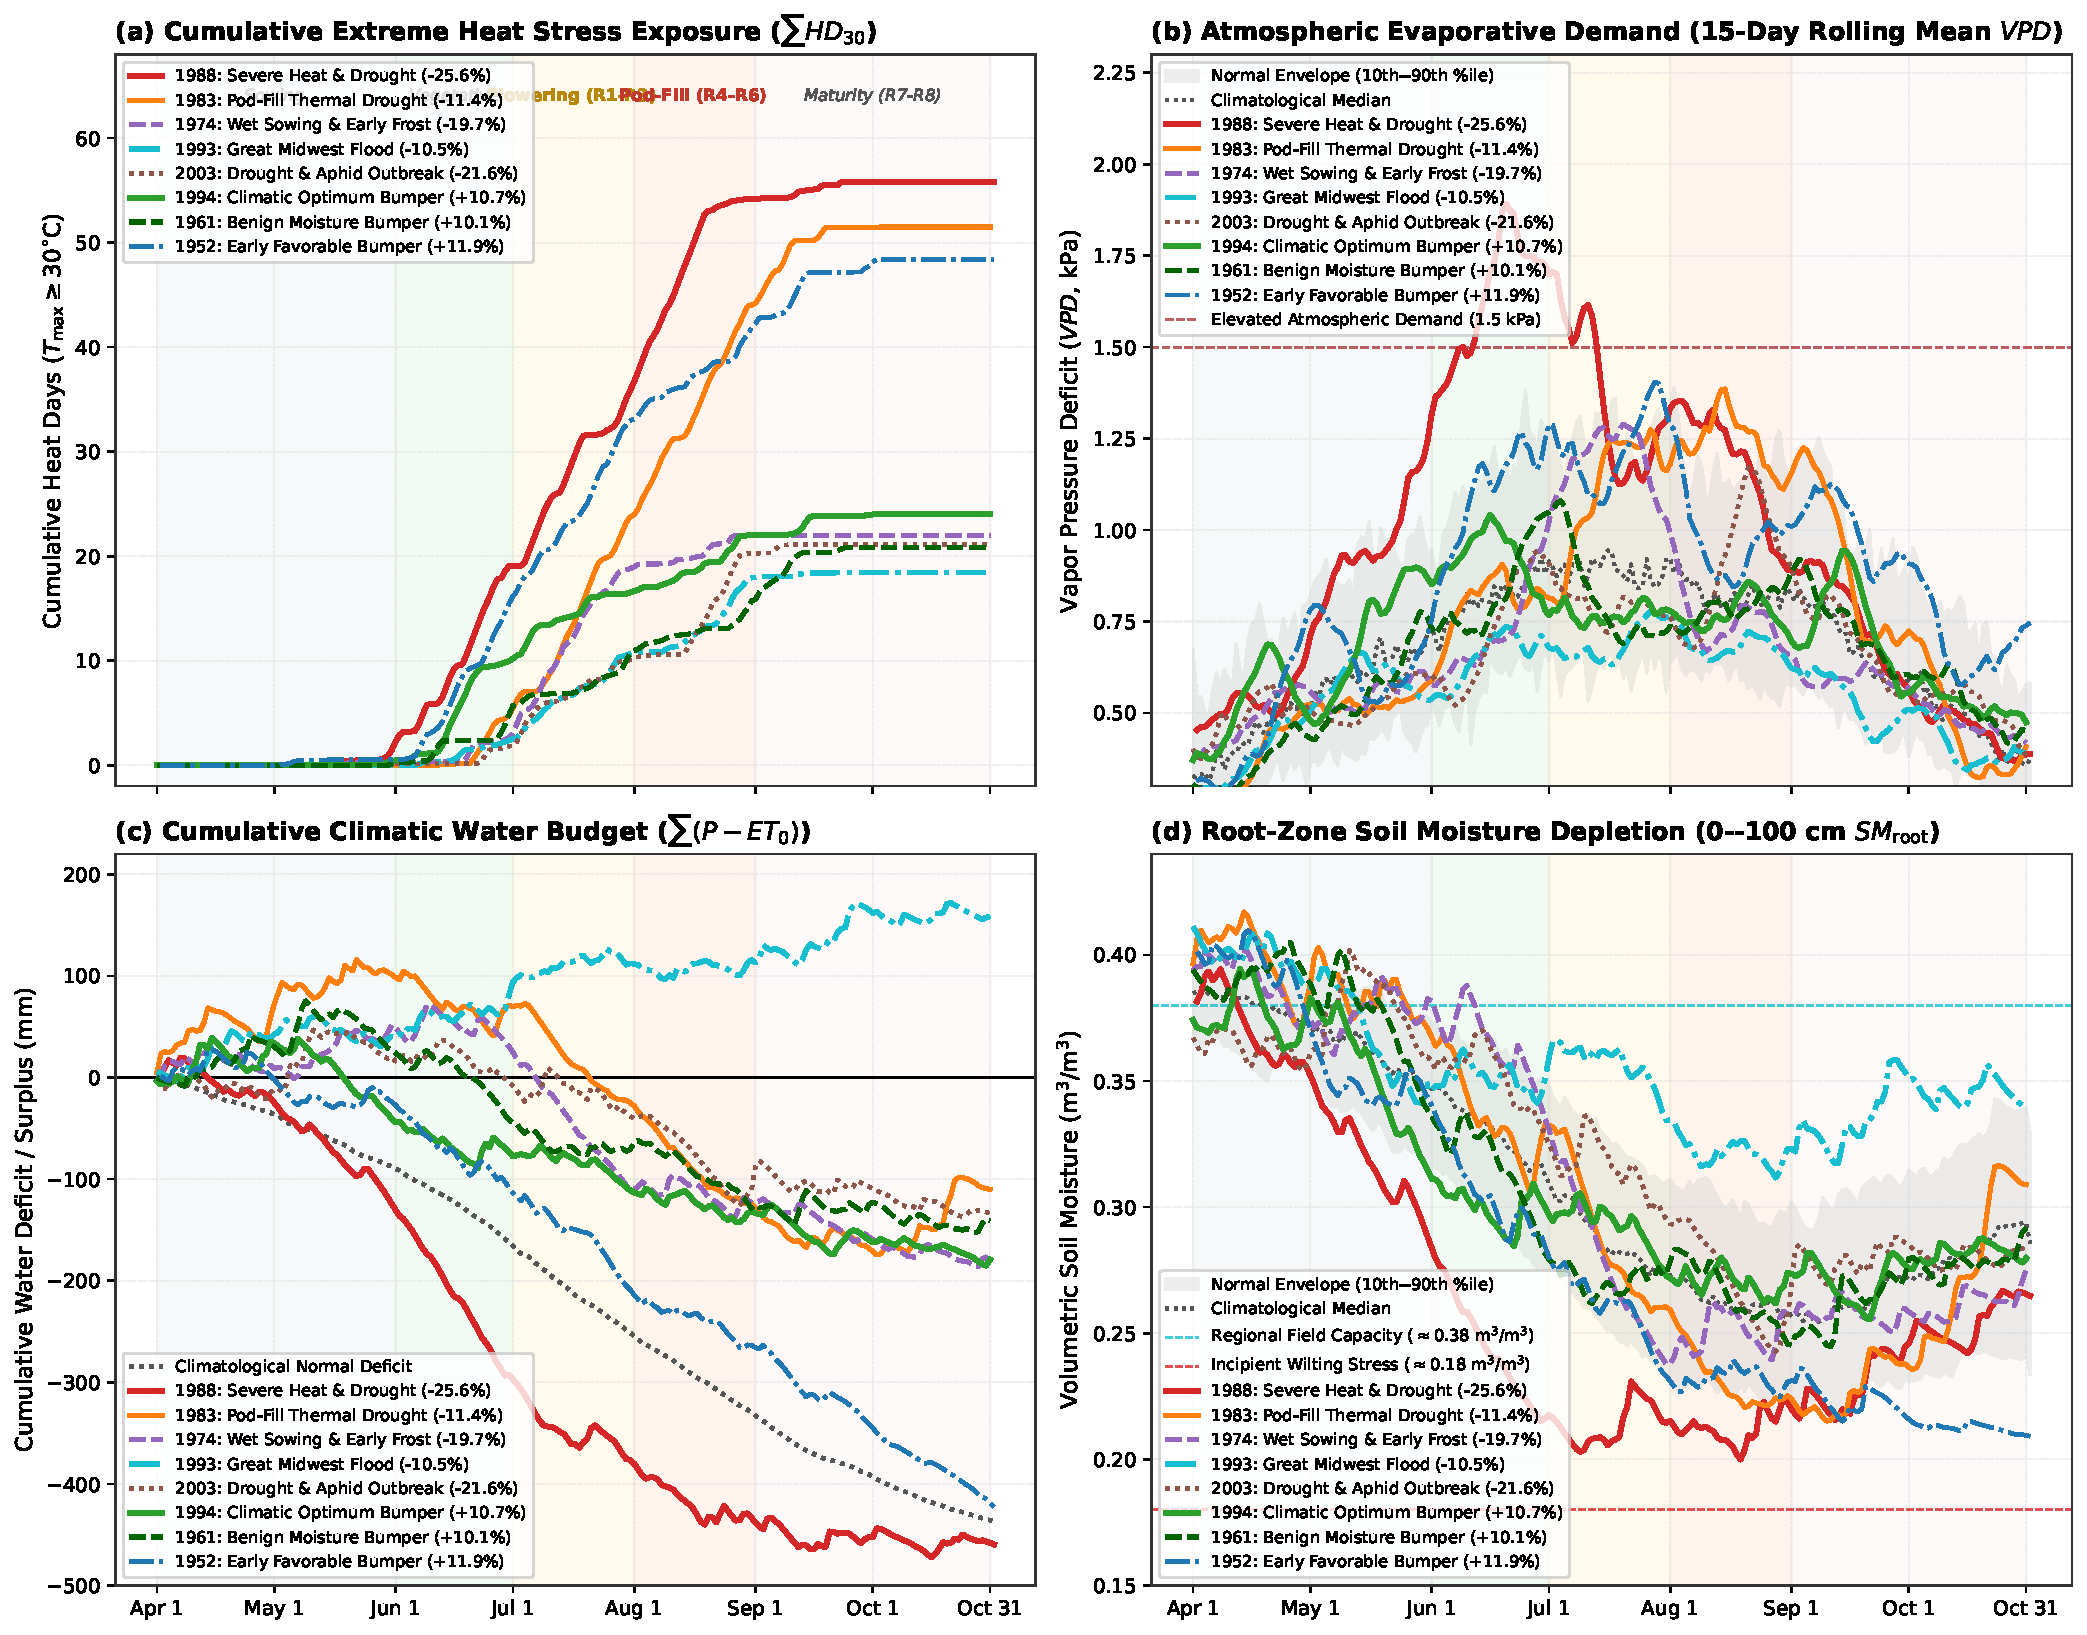
\includegraphics[width=0.96\textwidth]{figures/fig_intra_seasonal_extremes}
    \caption{Intra-seasonal phenological progression of historical extreme soybean yield years ($\pm 10\%$ threshold) across the Midwestern Corn Belt (April 1 to October 31). Panel (a) tracks cumulative extreme heat stress days ($\sum HD_{30}$, $T_{\text{max}} \ge 30^\circ\text{C}$). Panel (b) illustrates atmospheric evaporative demand via 15-day rolling mean $VPD$ against elevated demand ($1.5\text{ kPa}$) and the normal 10th--90th percentile envelope. Panel (c) traces the cumulative climatic water budget ($\sum (P - ET_0)$), contrasting catastrophic drought desiccation against flood waterlogging. Panel (d) displays depth-weighted root-zone soil moisture ($SM_{\text{root}}$, $0$--$100\text{ cm}$) against regional field capacity and incipient wilting stress. Trajectories distinguish individual negative shocks (1988, 1983, 1974, 1993, 2003) and positive bumper crops (1994, 1961, 1952).}
    \label{fig:intra_seasonal_extremes}
\end{figure}

\begin{figure}[htbp]
    \centering
    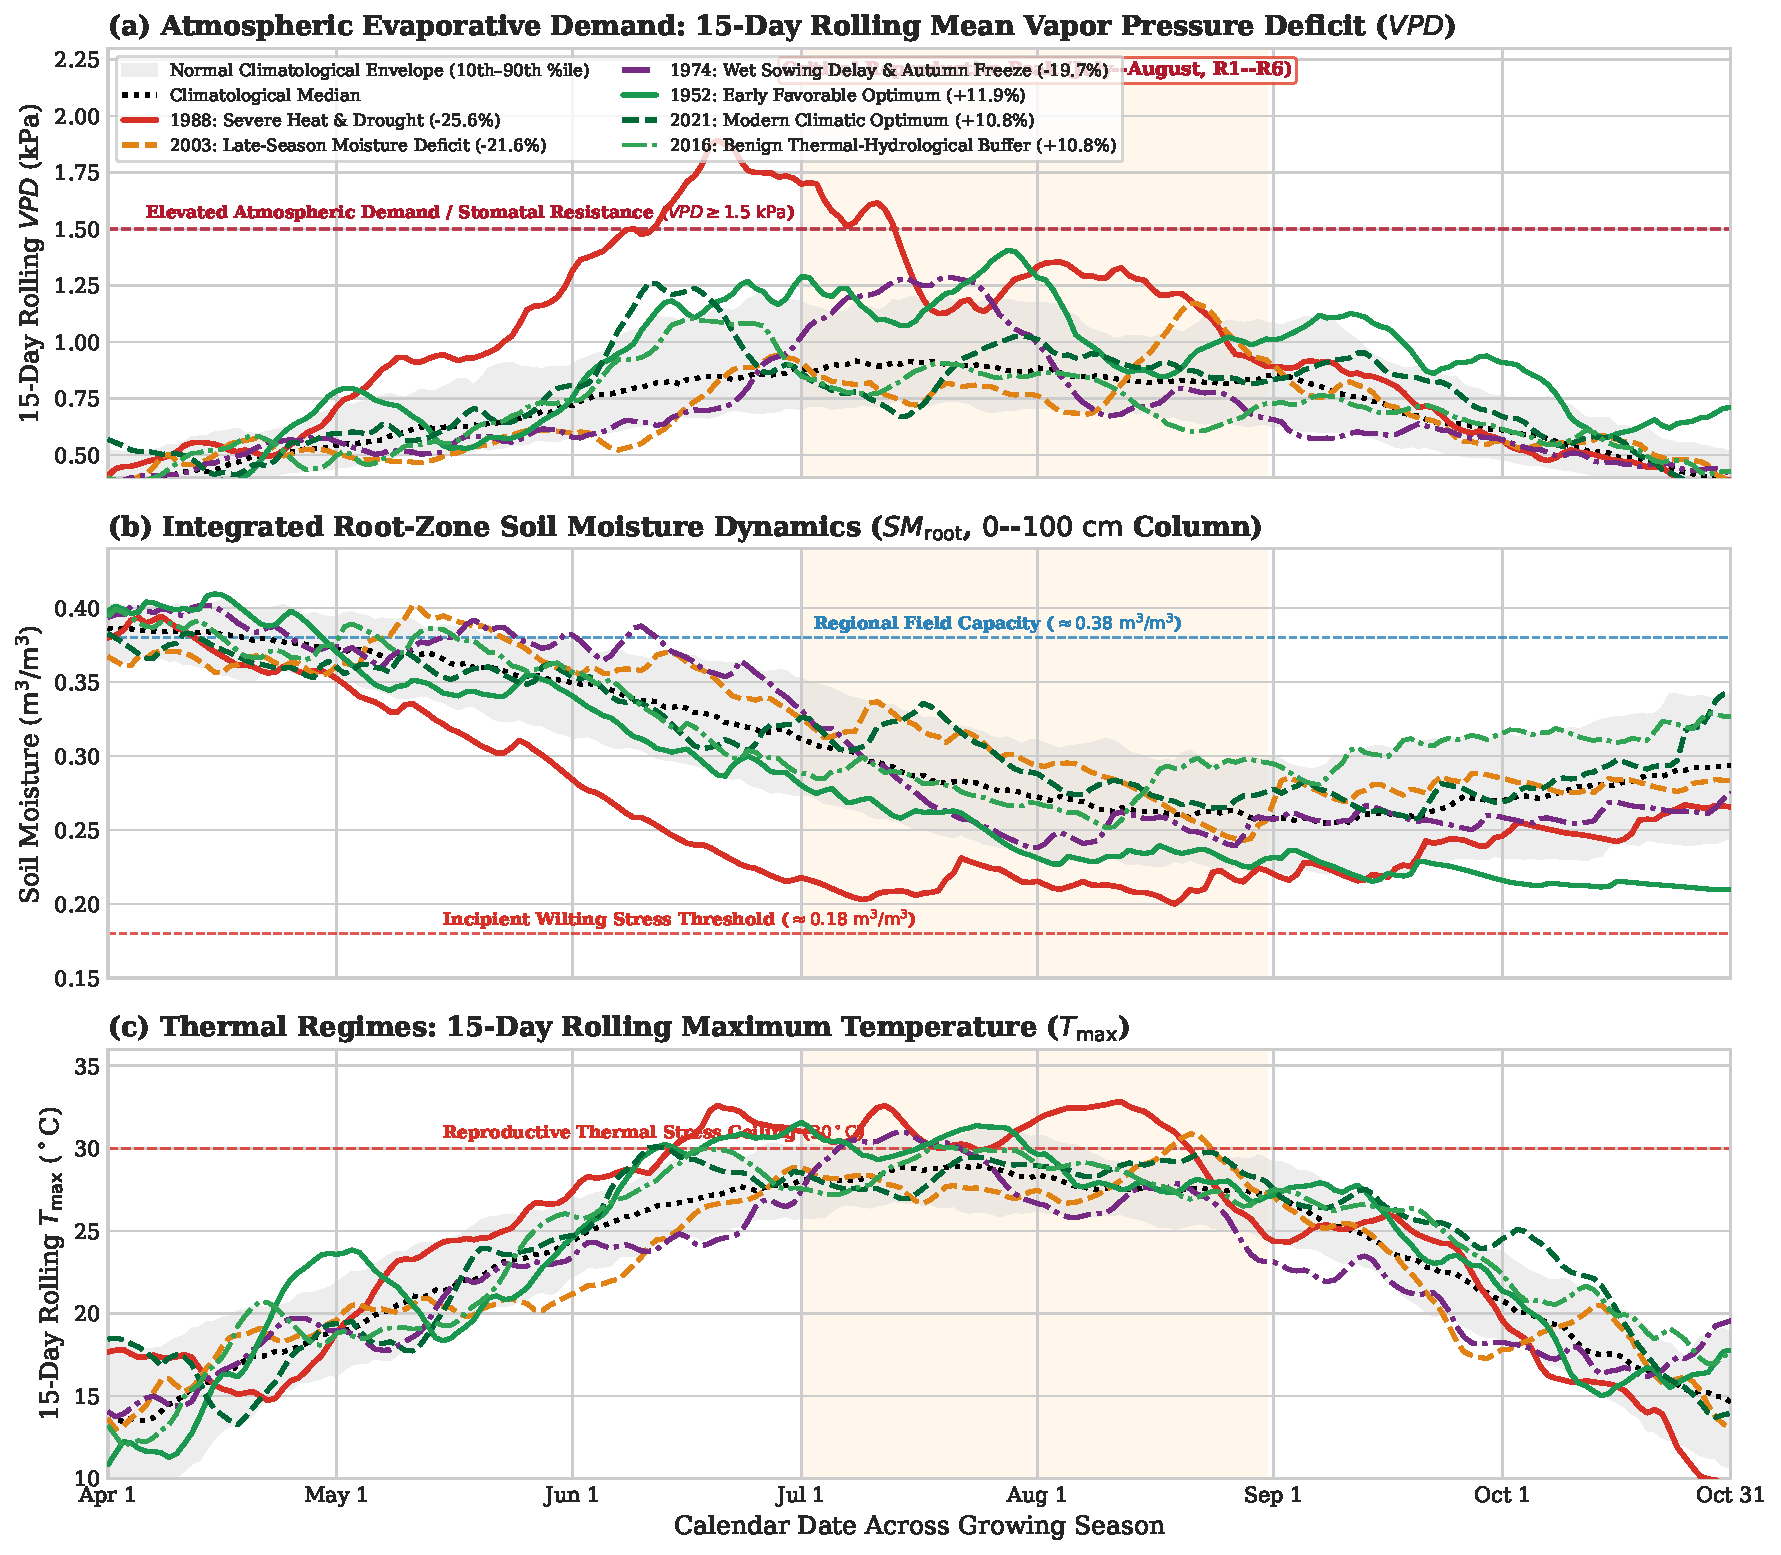
\includegraphics[width=0.96\textwidth]{figures/fig_weather_shocks_footprint}
    \caption{Comparative agro-climatic shock anomaly footprints across the soybean growing cycle (April--October) for representative historical archetypes: 1988 (severe summer heat and drought), 1983 (late-season pod-fill drought), 1974 (delayed wet sowing and early autumn freeze), 1993 (The Great Midwest Flood / soil waterlogging), and 1994 (climatic optimum / bumper harvest). Curves depict 15-day centered rolling anomalies relative to the historical panel climatology for precipitation ($P$), vapor pressure deficit ($VPD$), root-zone soil moisture ($SM_{\text{root}}$), and extreme heat days ($HD_{30}$).}
    \label{fig:weather_shocks_footprint}
\end{figure}

Synthesizing the daily trajectories and anomaly footprints reveals that historical extremes fall into four coherent agro-climatic cohorts:

\paragraph{Cohort I: Compound Thermal-Drought Stress.}
Drought-stressed campaigns across Midwestern history (including 1953, 1954, 1983, 1988, and 2012) are driven by persistent upper-tropospheric anticyclonic blocking ridges that displace frontal storm tracks northward. However, within this broad cohort, the daily trajectories resolve two critically distinct temporal stress profiles:
\begin{itemize}
    \item \textit{Chronic Full-Season Drought (e.g., 1988, 1953):} Meteorological deficits establish early in May and June, with rainfall anomalies running $-40$ to $-50\text{ mm/month}$ below normal throughout the summer (Figure~\ref{fig:weather_shocks_footprint}). Evaporative demand surges continuously ($VPD$ anomalies $> +0.8\text{ kPa}$), while heat-stress days accumulate steadily from mid-June to reach an unprecedented 56 days (Figure~\ref{fig:intra_seasonal_extremes}a). The cumulative climatic moisture deficit plunges below $-450\text{ mm}$, exhausting root-zone moisture reserves down to severe depletion levels ($<0.18\text{ m}^3/\text{m}^3$) well before seed filling, causing stunted vegetative frames and massive flower abortion.
    \item \textit{Reproductive Flash Drought and Pod-Fill Collapse (e.g., 1983, 2012):} In sharp contrast, vegetative development through May and June experiences near-normal rainfall and moderate temperatures, fostering expansive canopy development and high transpirational demand. In late July, however, an abrupt synoptic blocking ridge collapses precipitation to near zero and triggers an acute thermal surge ($HD_{30} > +5\text{ days/month}$, $VPD > +0.7\text{ kPa}$) directly coincident with pod fill (R4--R6, Figure~\ref{fig:weather_shocks_footprint}). The lush vegetative biomass rapidly drains remaining subsoil moisture, precipitating severe pod abortion, incomplete pod filling, and shriveled grain. These dynamics confirm that robust vegetative vigor offers zero buffer against acute late-season moisture deficits.
\end{itemize}

\paragraph{Cohort II: Pluvial Excess and Hydrological Saturation.}
Pluvial disaster seasons across the historical record (e.g., 1958, 1993, 2008, 2015) exhibit physical trajectories that represent the polar antithesis of drought. Cumulative heat days plateau at minimal levels ($\sum HD_{30} < 18\text{ days}$), while high relative humidity and cloud cover depress $VPD$ to $0.50$--$0.75\text{ kPa}$ (Figure~\ref{fig:intra_seasonal_extremes}a,b). Instead, persistent zonal storm tracks generate immense rainfall surpluses ($+60$ to $+100\text{ mm/month}$ above normal, Figure~\ref{fig:weather_shocks_footprint}), driving cumulative $P - ET_0$ past $+160\text{ mm}$. Root-zone soil moisture remains pinned at absolute saturation ($>0.40\text{ m}^3/\text{m}^3$). This sustained inundation suffocates root respiration, impairs symbiotic rhizobial nitrogen fixation, fosters extensive Phytophthora root rots, and leaves heavy machinery unable to enter saturated fields.

\paragraph{Cohort III: Temporal Boundary and Cold Truncation Hazards.}
Seasons governed by temporal boundary shocks (e.g., 1974, 2019) demonstrate that agricultural productivity can be severely impaired without anomalous midsummer heat or midsummer drought. In these campaigns, torrential spring precipitation saturates topsoils throughout April and May, delaying regional sowing operations by 3--4 weeks into June (Figure~\ref{fig:intra_seasonal_extremes}c). While midsummer temperatures and water balances remain moderate, this operational delay shifts the reproductive pod-fill calendar late into August and September. In late September, an unseasonably early Arctic cold front brings hard sub-freezing temperatures ($T_{\text{min}} < -2^\circ\text{C}$) across the northern and central Corn Belt (Figure~\ref{fig:weather_shocks_footprint}). The freeze abruptly kills the canopy before physiological maturity (R7), arresting carbohydrate translocation and permanently freezing immature green seeds in their pods.

\paragraph{Cohort IV: Agro-Climatic Optima and Bumper Harvest Regimes.}
Prominent bumper harvest cohorts across diverse technological eras (e.g., 1952, 1961, 1979, 1994, 2016, 2021) follow an ideal agro-climatic middle path. Daily temperatures remain remarkably mild, with daytime maxima consistently below $28^\circ\text{C}$ and cumulative heat-stress days plateauing below 20 days (Figure~\ref{fig:intra_seasonal_extremes}a). Atmospheric evaporative demand hovers smoothly within the transpirational optimum ($VPD \approx 0.75$--$1.0\text{ kPa}$), preventing midday stomatal closure while supporting vigorous carbon assimilation. Crucially, timely and well-distributed convective rainfall events replenish root-zone soil moisture at regular 7- to 10-day intervals without creating waterlogged conditions, maintaining $SM_{\text{root}}$ securely between $0.27$ and $0.34\text{ m}^3/\text{m}^3$ throughout the critical August seed-filling window (Figure~\ref{fig:intra_seasonal_extremes}d). Under these benign conditions, crops achieve the maximum photosynthetic yield permitted by the biological ceiling of C3 RuBisCO kinetics.

\subsection{Phenological Climate-Yield Sensitivity and Lead-Time Dynamics}
\label{sec:data_pheno_sensitivity}

To quantify the evolving empirical dependency between atmospheric anomalies and county soybean yields across the growing season, Figure~\ref{fig:climate_yield_sensitivity} presents bivariate Pearson correlation coefficients ($r$) computed between detrended yield anomalies ($\epsilon_{c,t}$) and monthly atmospheric anomalies across the 135 study counties.

\begin{figure}[htbp]
    \centering
    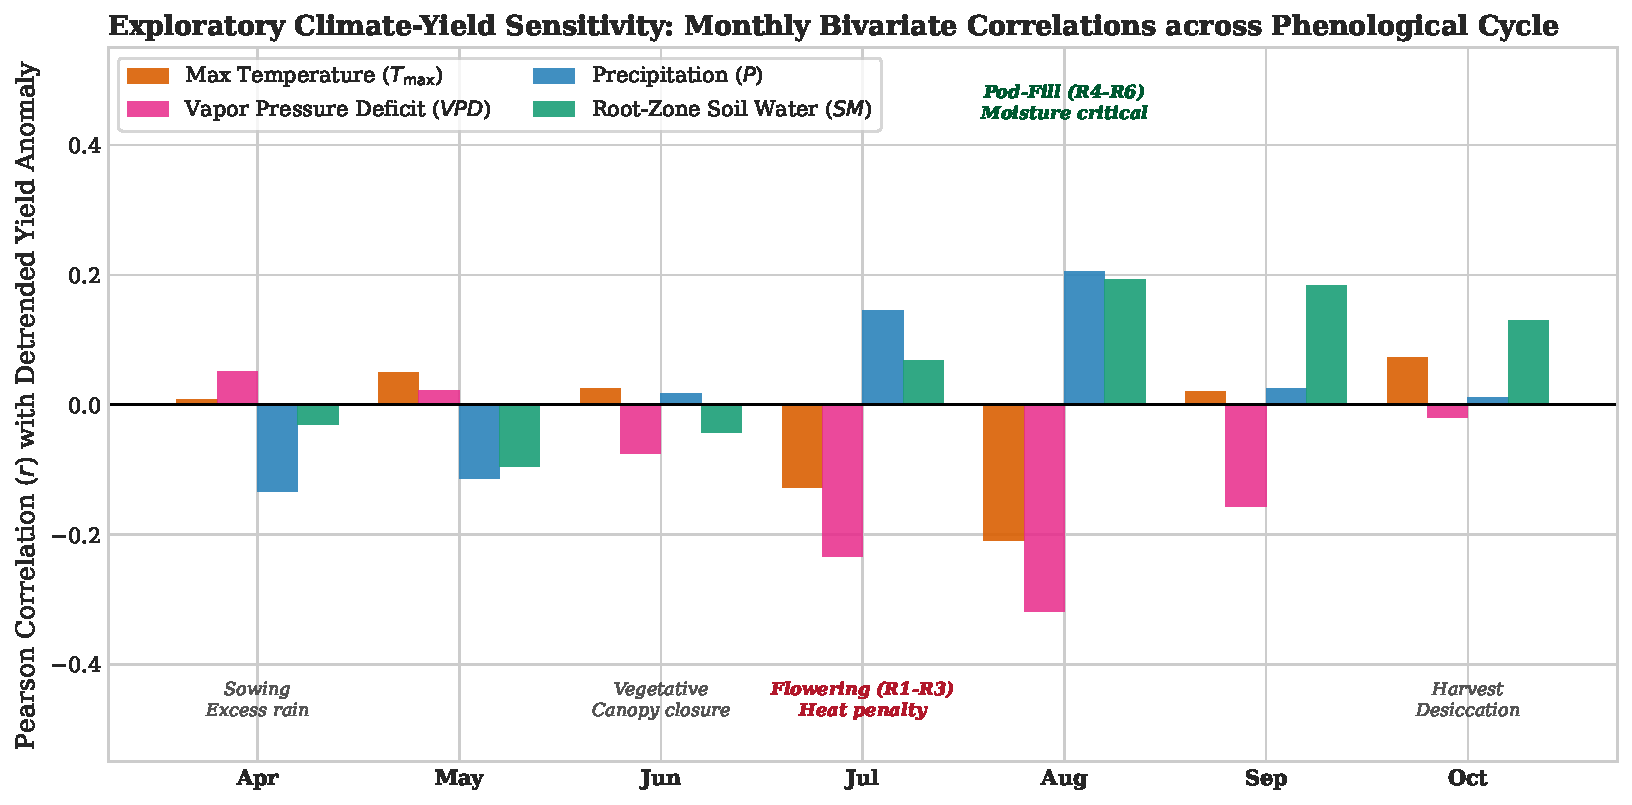
\includegraphics[width=0.96\textwidth]{figures/fig_climate_yield_sensitivity}
    \caption{Phenological sensitivity of county soybean yields to monthly atmospheric anomalies across the crop cycle (April--October). Bars depict cross-sectional Pearson correlation coefficients ($r$) between detrended yield anomalies ($\epsilon_{c,t}$) and monthly anomalies of maximum temperature ($T_{\text{max}}$), vapor pressure deficit ($VPD$), precipitation ($P$), and root-zone soil moisture ($SM_{\text{root}}$). Yield sensitivity is minimal during pre-sowing and emergence (April--May), escalates sharply during flowering (July), peaks during pod filling (August), and decays rapidly upon physiological maturity (September--October).}
    \label{fig:climate_yield_sensitivity}
\end{figure}

The empirical sensitivity profiles display four distinct phenological stages:
\begin{enumerate}
    \item \textbf{Pre-Sowing and Emergence Window (April--May):} Correlation coefficients between yield anomalies and weather variables are uniformly low ($|r| < 0.10$). Notably, precipitation and soil moisture exhibit slightly negative correlations with final yield ($r \approx -0.06$ to $-0.09$). This counter-intuitive negative relationship reflects the operational penalties of excessive spring moisture: wet fields delay field preparation and seeding, promote soil compaction, and foster early seedling diseases. Ambient temperature exerts negligible influence during this preparatory phase.
    \item \textbf{Vegetative Growth and Canopy Closure (June):} As crops establish root systems and leaf area, the sign of environmental sensitivities shifts toward positive moisture dependency. However, correlation magnitudes remain moderate ($r \approx +0.12$ for soil moisture; $r \approx -0.14$ for $VPD$), indicating that soybeans possess sufficient vegetative plasticity to recover from early-season weather aberrations if subsequent reproductive conditions are favorable.
    \item \textbf{Peak Reproductive Sensitivity (July--August):} Atmospheric sensitivity escalates dramatically during flowering (July, R1--R3) and reaches its maximum amplitude during pod development and seed filling (August, R4--R6). In August, the correlation between yield anomalies and root-zone soil moisture surges to $r = +0.43$, accompanied by precipitation at $r = +0.38$. Concurrently, atmospheric stress metrics exhibit severe negative correlations: $VPD$ reaches $r = -0.46$ and $T_{\text{max}}$ reaches $r = -0.41$. The co-occurrence of maximum evaporative demand ($VPD$) and reproductive seed swelling makes August weather the single most critical determinant of interannual yield variance.
    \item \textbf{Maturation and Senescence (September--October):} Following the completion of seed fill in late August, soybean leaves undergo rapid monocarpic senescence and yellowing (R7), followed by physiological maturity (R8) and field dry-down. Consequently, correlation coefficients plunge precipitously back toward zero ($|r| \le 0.05$ across all four variables). Atmospheric conditions in September and October affect grain moisture content and combine harvest efficiency, but exert zero biological impact on realized seed quantity.
\end{enumerate}

\paragraph{Methodological Implications for Progressive Lead-Time Forecasting.} The empirical sensitivity dynamics synthesized in Figure~\ref{fig:climate_yield_sensitivity} provide the direct scientific foundation for the progressive lead-time forecasting framework formalized in Chapter~4. 

At long presowing lead times ($H = 12, \dots, 6$, October through April), atmospheric forcings exhibit low direct correlation with final yield anomalies; predictive skill at these horizons must rely primarily on persistent antecedent root-zone soil moisture recharge and multi-month hydrological memory \citep{Vijverberg2023}. As the forecast horizon advances through vegetative development ($H = 5, 4$, May and June), incoming meteorological information gradually updates crop potential, but the system remains subject to high downstream epistemic uncertainty. 

The primary leap in physical predictability occurs at mid-season and late-summer horizons ($H = 3, 2$, July 31 and August 31), when predictive models ingest the realized atmospheric stress profile during the critical flowering and pod-fill windows. Finally, at horizon $H = 1$ (September 30), the biological crop yield is essentially fixed; remaining forecast uncertainty is dominated by localized combine harvest losses and late frost hazards rather than physiological yield formation. The mathematical formalization of these twelve discrete forecasting horizons, alongside the multi-granularity feature extraction and expanding-window validation protocols, is developed in Chapter~4.

